\begin{frame}\frametitle{Strategy}
\centering\myskip

\begin{minipage}{.25\textwidth}\centering
\footnotesize

$\TTbar\to Ht+X$

\myskip

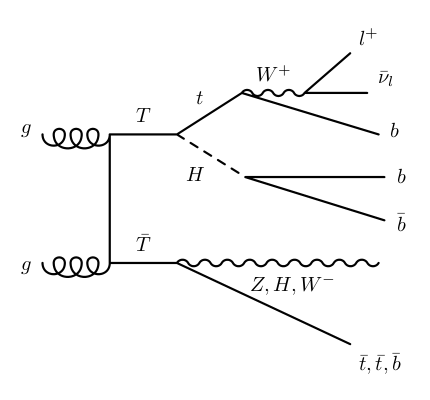
\includegraphics[width=1.15\textwidth]{pics/feyn_htX}

%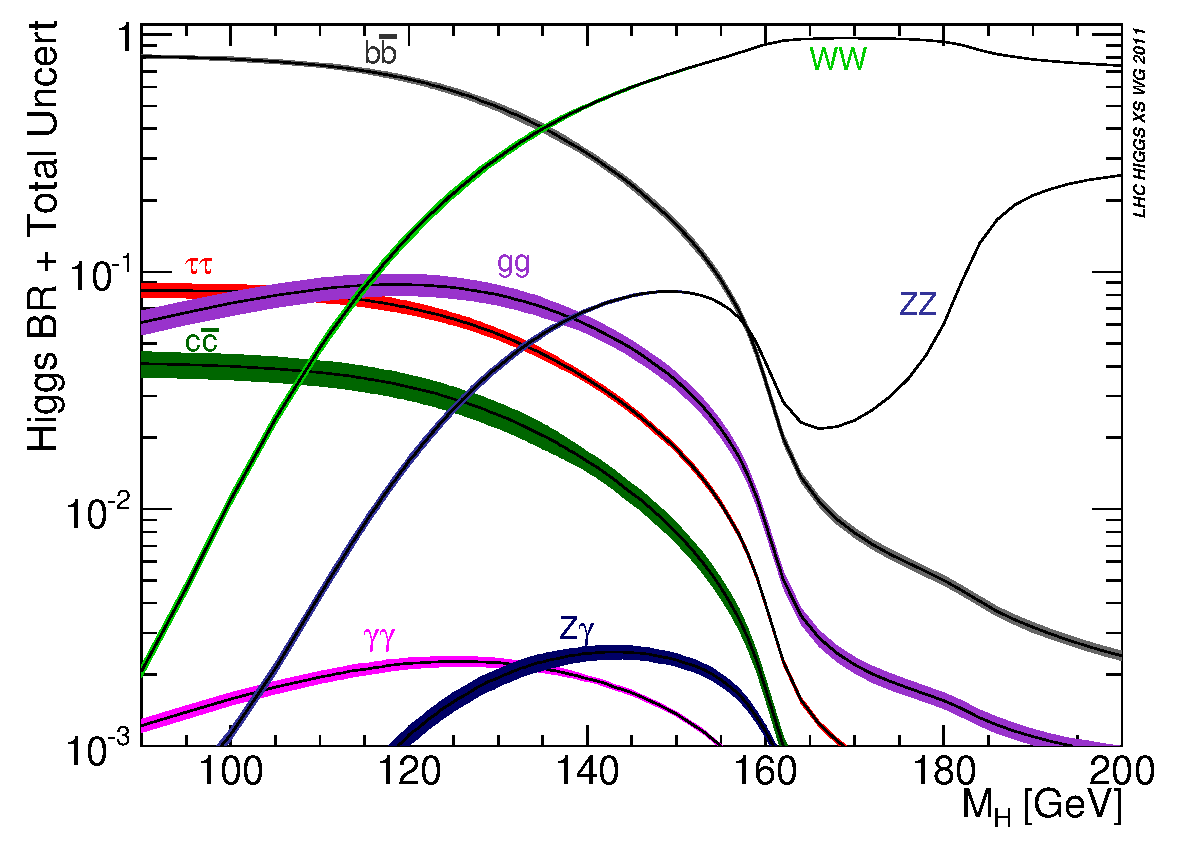
\includegraphics[width=1.15\textwidth]{pics/BRTotalUncertBands_lm}
SM Higgs boson\\
w/ {\cccolor $m_H=125\gev$}\\
$\Downarrow$\\
BR($H\to bb$) = 60\%\\
BR($H\to WW$) = 20\%\\



\end{minipage}\begin{minipage}{.75\textwidth}\centering
\footnotesize
\vskip-5ex

\begin{tabular}{p{.7cm}ll}
  \multirow{2}{*}{$T\to Ht$} & {\tiny$\nearrow$} $bbWb \to bbbl\nu$ & \multirow{2}{*}{+ $\bar{T}\to Wb/Zt/Ht$}\\
                             & {\tiny$\searrow$} $WWWb \to qqqqbl\nu$&\\
\end{tabular}

\myskip

as a minimum {\cccolor 6} total jets in the event ($\TTbar\to HtWb$)\\
{\LARGE $\Downarrow$}\\
$\HT = \pT(l) + \met + \sum_{j = 1}^{\rm N jets}\pT(j)$\\

\scriptsize
\myskip
{\cccolor peak $\sim 2m_T$}\\
good signal/bkg discriminant $\qquad$ for all $Ht+X$ modes


\hskip5ex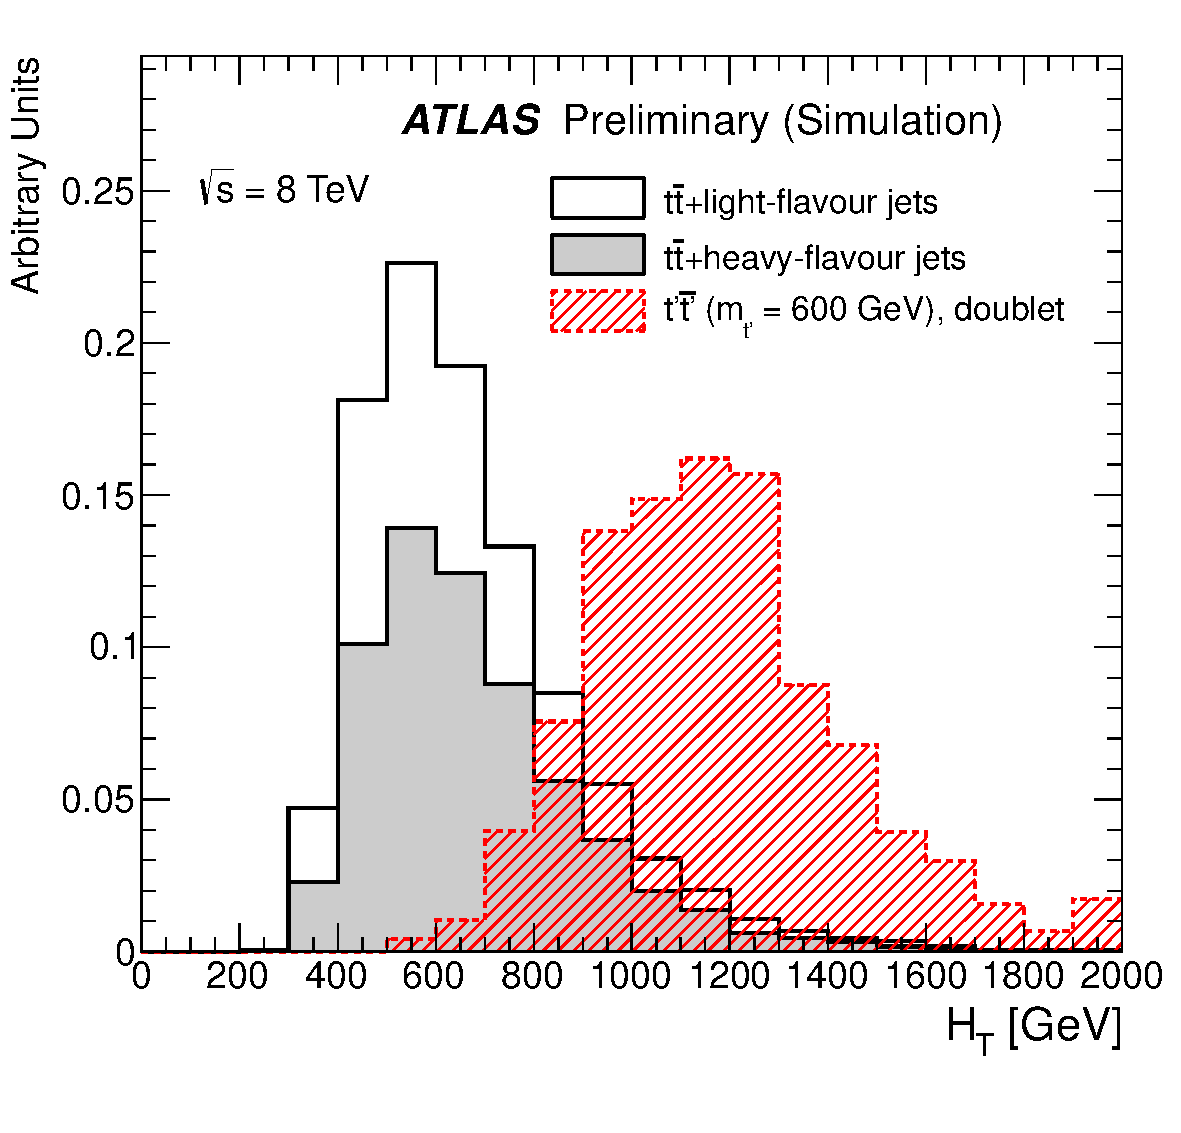
\includegraphics[width=.45\textwidth]{pics/HTAll_ELEMUON_6jetin4btagin_NOMINAL_VLTtt}
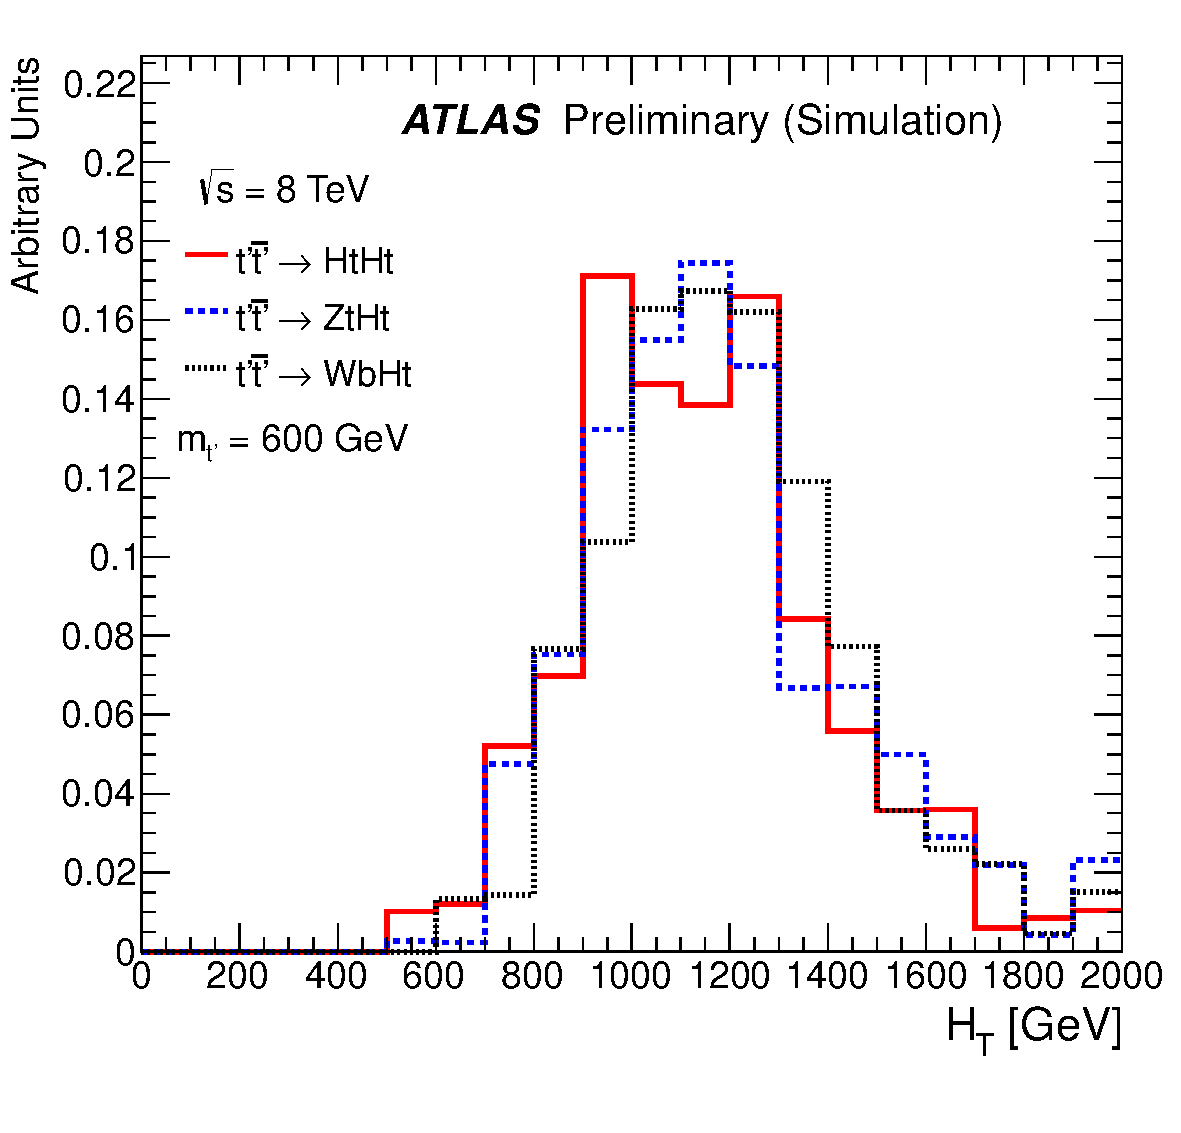
\includegraphics[width=.45\textwidth]{pics/HTAll_ELEMUON_6jetin4btagin_NOMINAL_decaysVLT}

$\geq 6$ jets, $\geq 4$ \bjet s

\end{minipage}

\end{frame}


%%%%%%%%%%%%%%%%%%%%%%%%%
%%%
%%%%%%%%%%%%%%%%%%%%%%%%%
\begin{frame}\frametitle{Event selection}
\centering\footnotesize

\begin{minipage}{.5\textwidth}\centering\scriptsize

\myskip

\begin{tabular}{ll}
\toprule
\pchii\  & $\geq 6$ jets\\
 & =2 $b$-tagged jets \\
 & \cccolor orthogonality cut: \\
 & $\HT < 700~\gev$ \\
\midrule
\pchiii\  & $\geq 6$ jets\\
&  =3 $b$-tagged jets \\
\midrule
\pchiv\  &$\geq 6$ jets\\
& $\geq 4$ $b$-tagged jets \\
\bottomrule
\end{tabular}

\myskip

\end{minipage}\begin{minipage}{.5\textwidth}\centering

%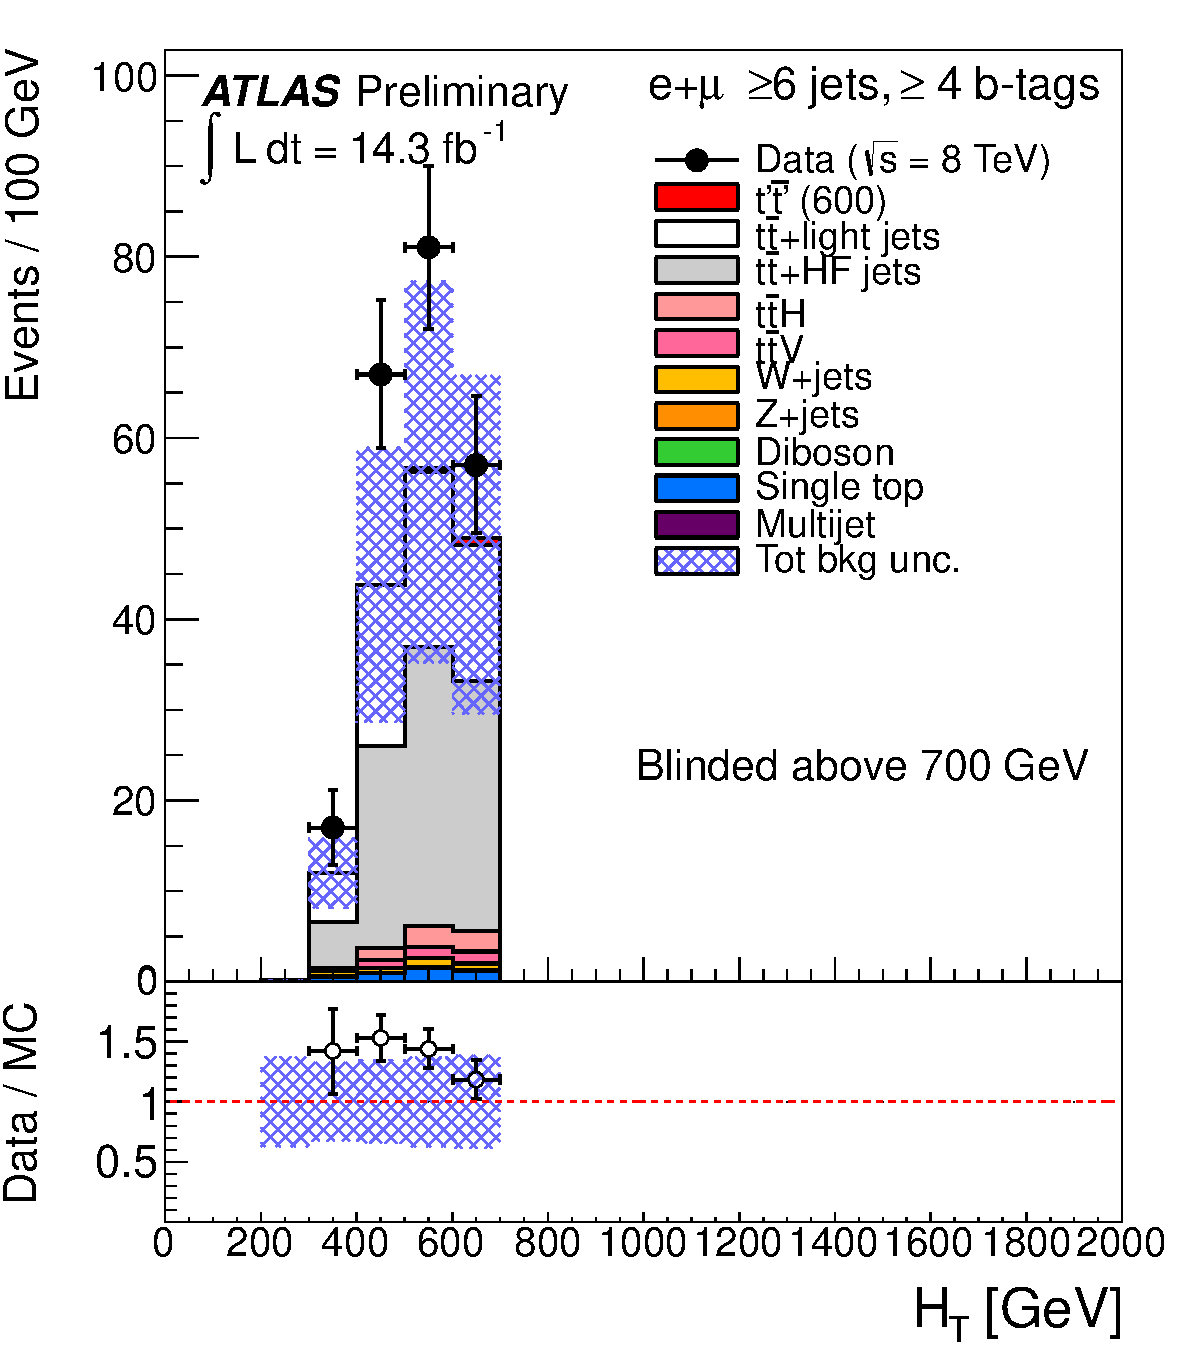
\includegraphics[width=.8\textwidth]{pics/htx_unscaled/HTAll_ELEMUON_6jetin4btagin_NOMINAL.pdf}

Consider three \bjet s multiplicities:
\begin{itemize}
\item maximize signal acceptance
\item insight on the heavy- and light-flavor components
\end{itemize}

each channel has a very different fraction of \tthf\ and \ttlf



\end{minipage}


\end{frame}


%%%%%%%%%%%%%%%%%%%%%%%%%
%%%
%%%%%%%%%%%%%%%%%%%%%%%%%
\begin{frame}\frametitle{Scale of \ttbar\ components}
\centering\footnotesize

heavy flavor component not well predicted\\ 
$\Downarrow$ \\ 
simultaneous fit to data of \HT\ variable\\
%(good to have {\cccolor background enriched} channels)

 \ttlf: $0.87 \pm 0.02\,{\rm (stat.)} \qquad$  \tthf: $1.35 \pm 0.11\,{\rm (stat.)}$

\myskip
\only<1>{
before\dots\\
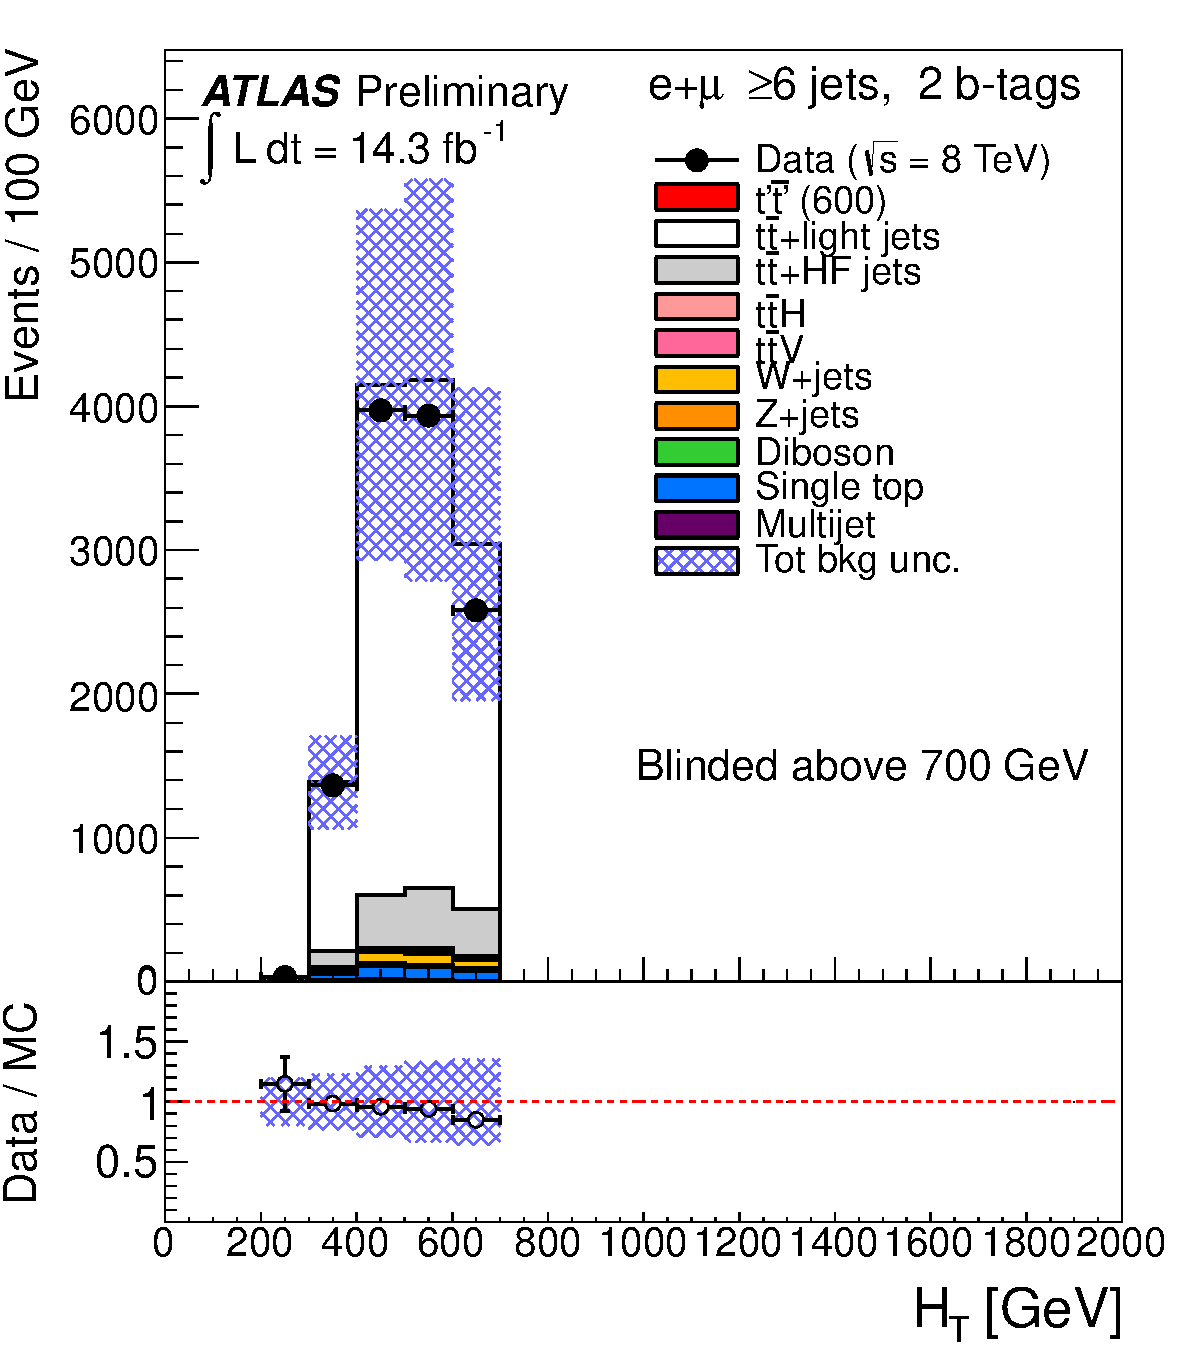
\includegraphics[width=.3\textwidth]{pics/htx_unscaled/HTAll_ELEMUON_6jetin2btagex_NOMINAL.pdf}
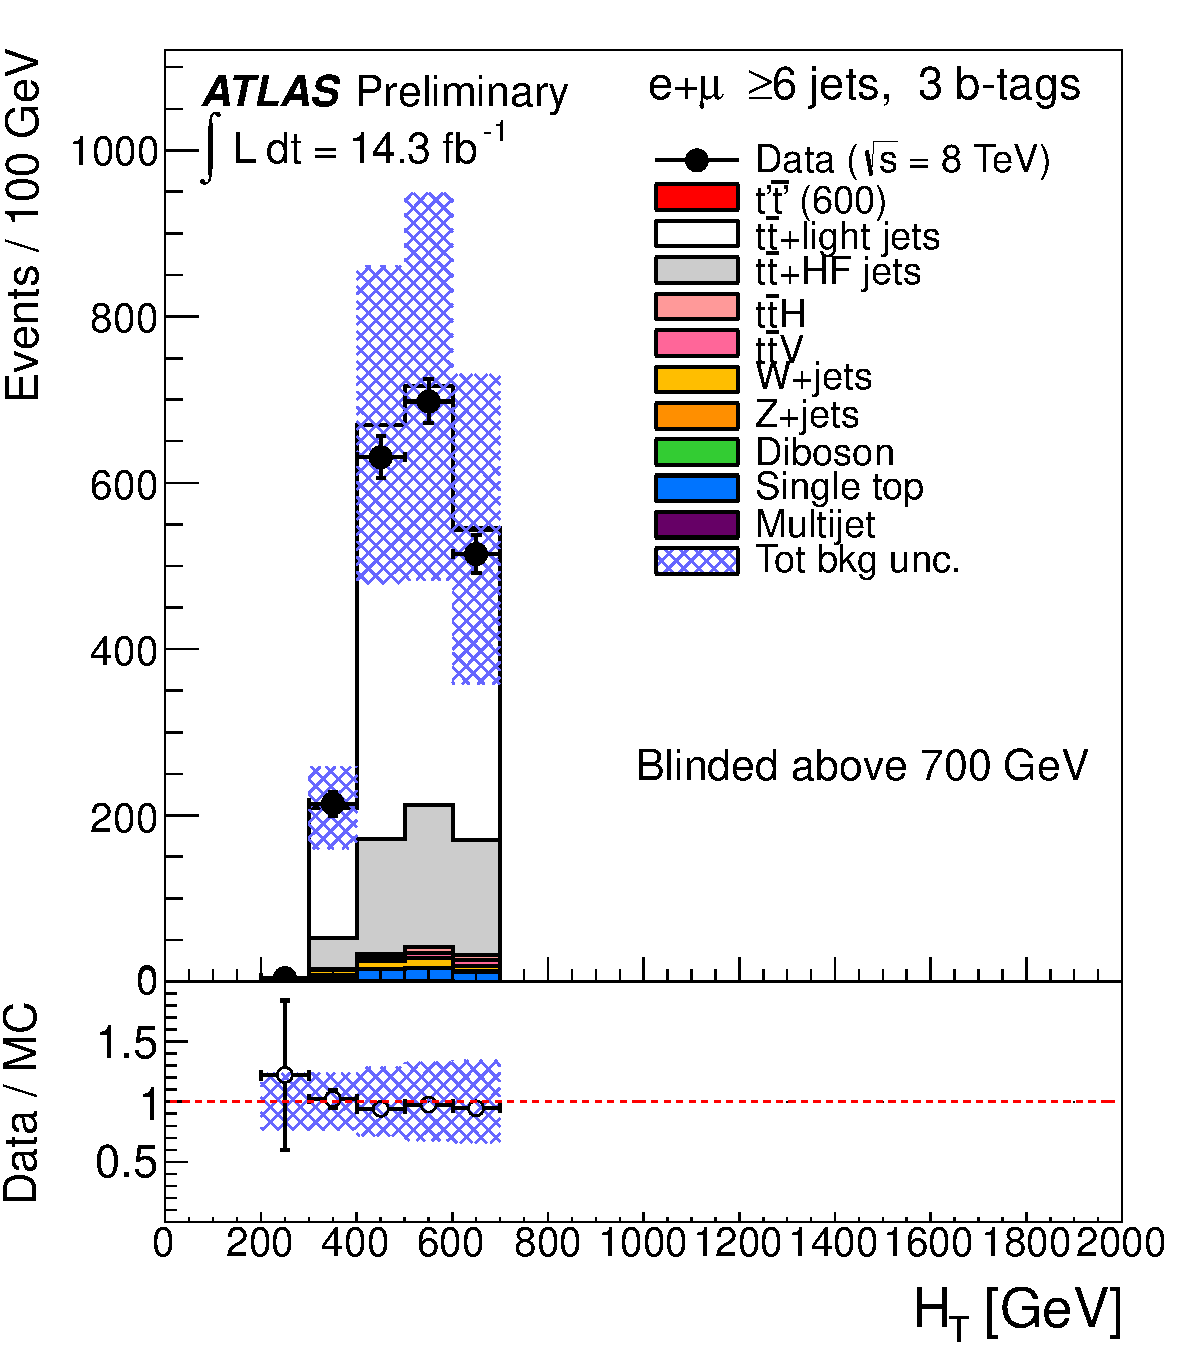
\includegraphics[width=.3\textwidth]{pics/htx_unscaled/HTAll_ELEMUON_6jetin3btagex_NOMINAL.pdf}
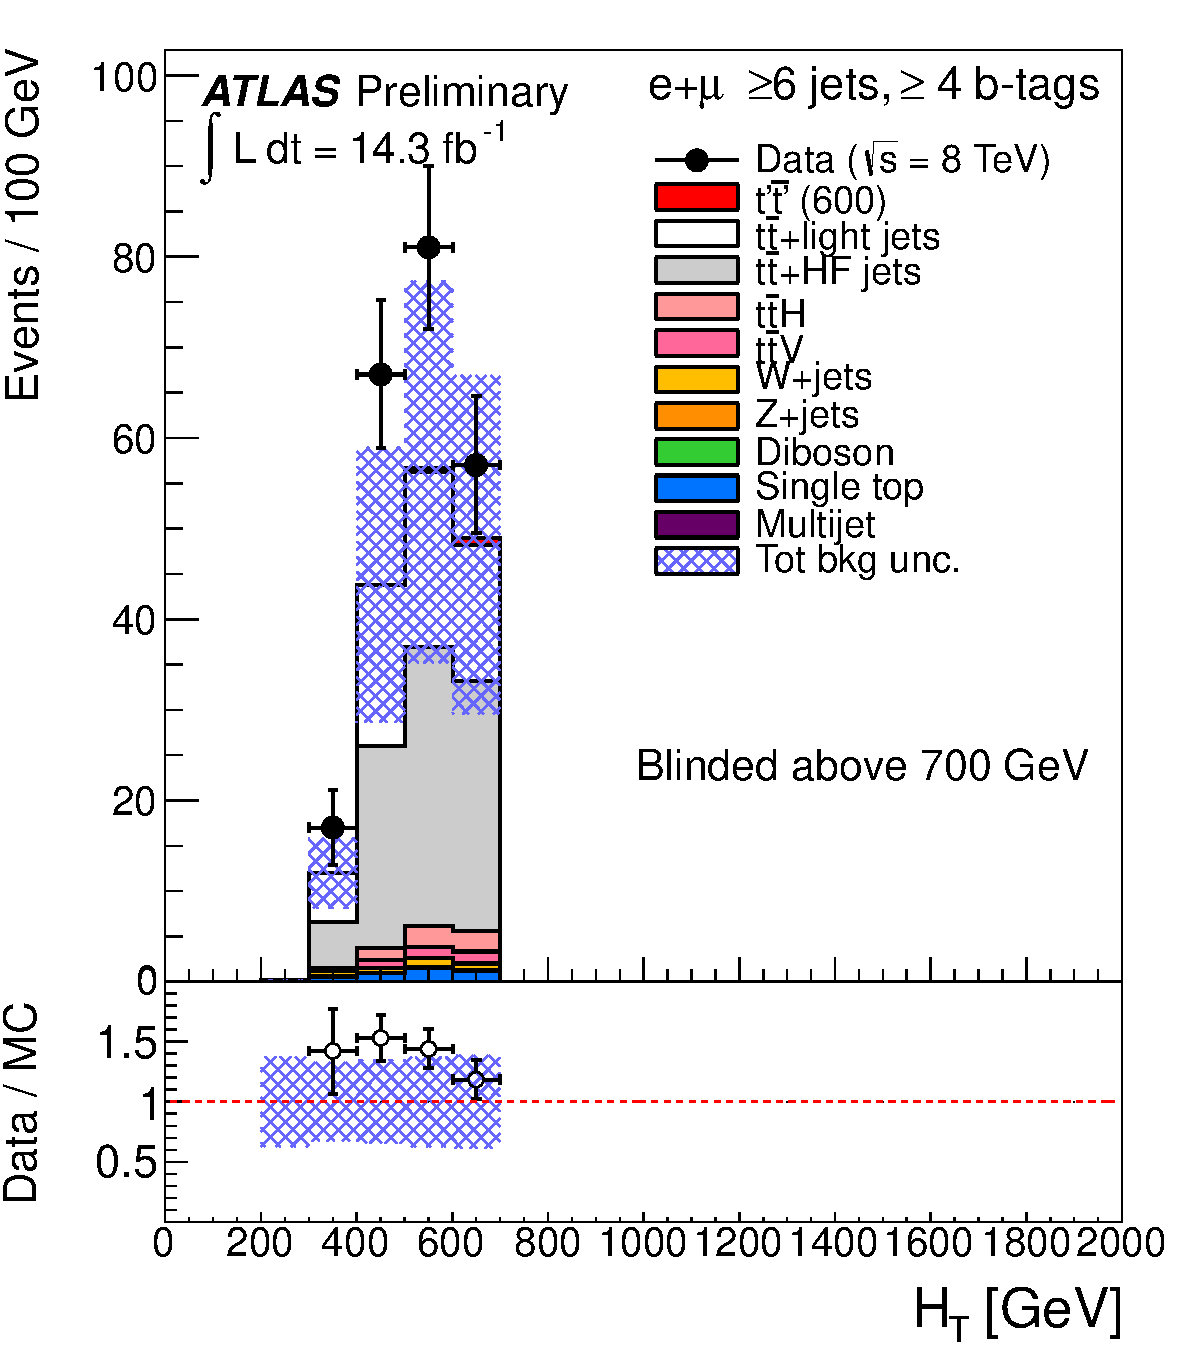
\includegraphics[width=.3\textwidth]{pics/htx_unscaled/HTAll_ELEMUON_6jetin4btagin_NOMINAL.pdf}
}\only<2>{
\dots after\\
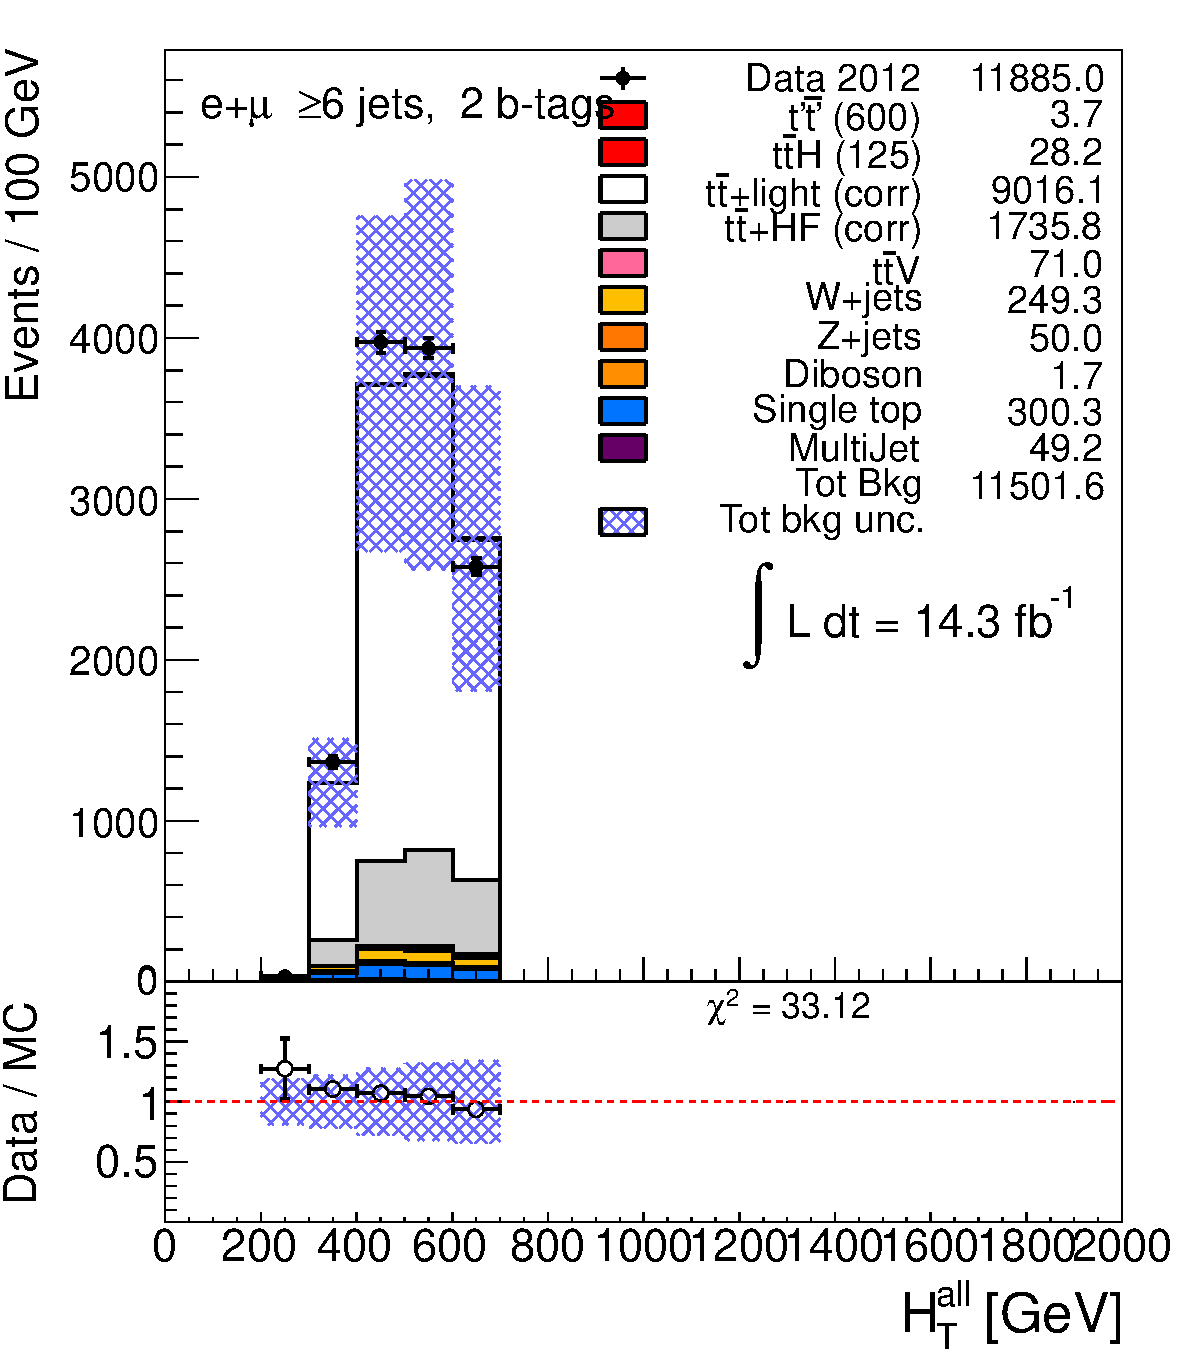
\includegraphics[width=.3\textwidth]{pics/htx_scaled/HTAll_ELEMUON_6jetin2btagex_NOMINAL.pdf}
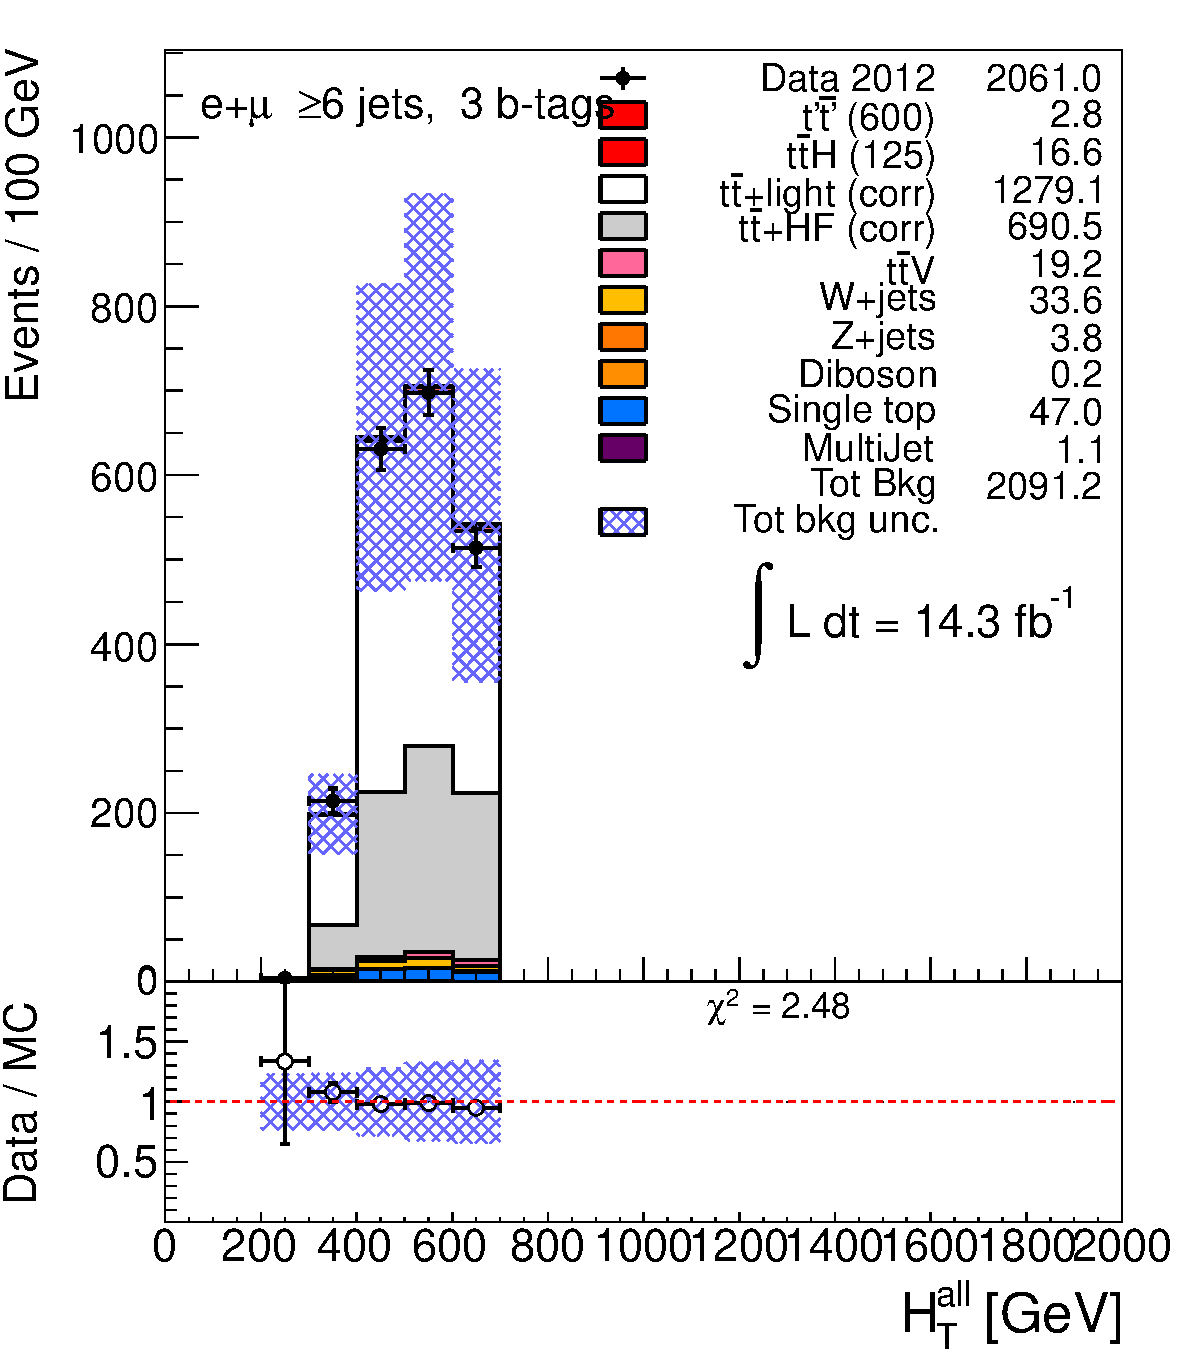
\includegraphics[width=.3\textwidth]{pics/htx_scaled/HTAll_ELEMUON_6jetin3btagex_NOMINAL.pdf}
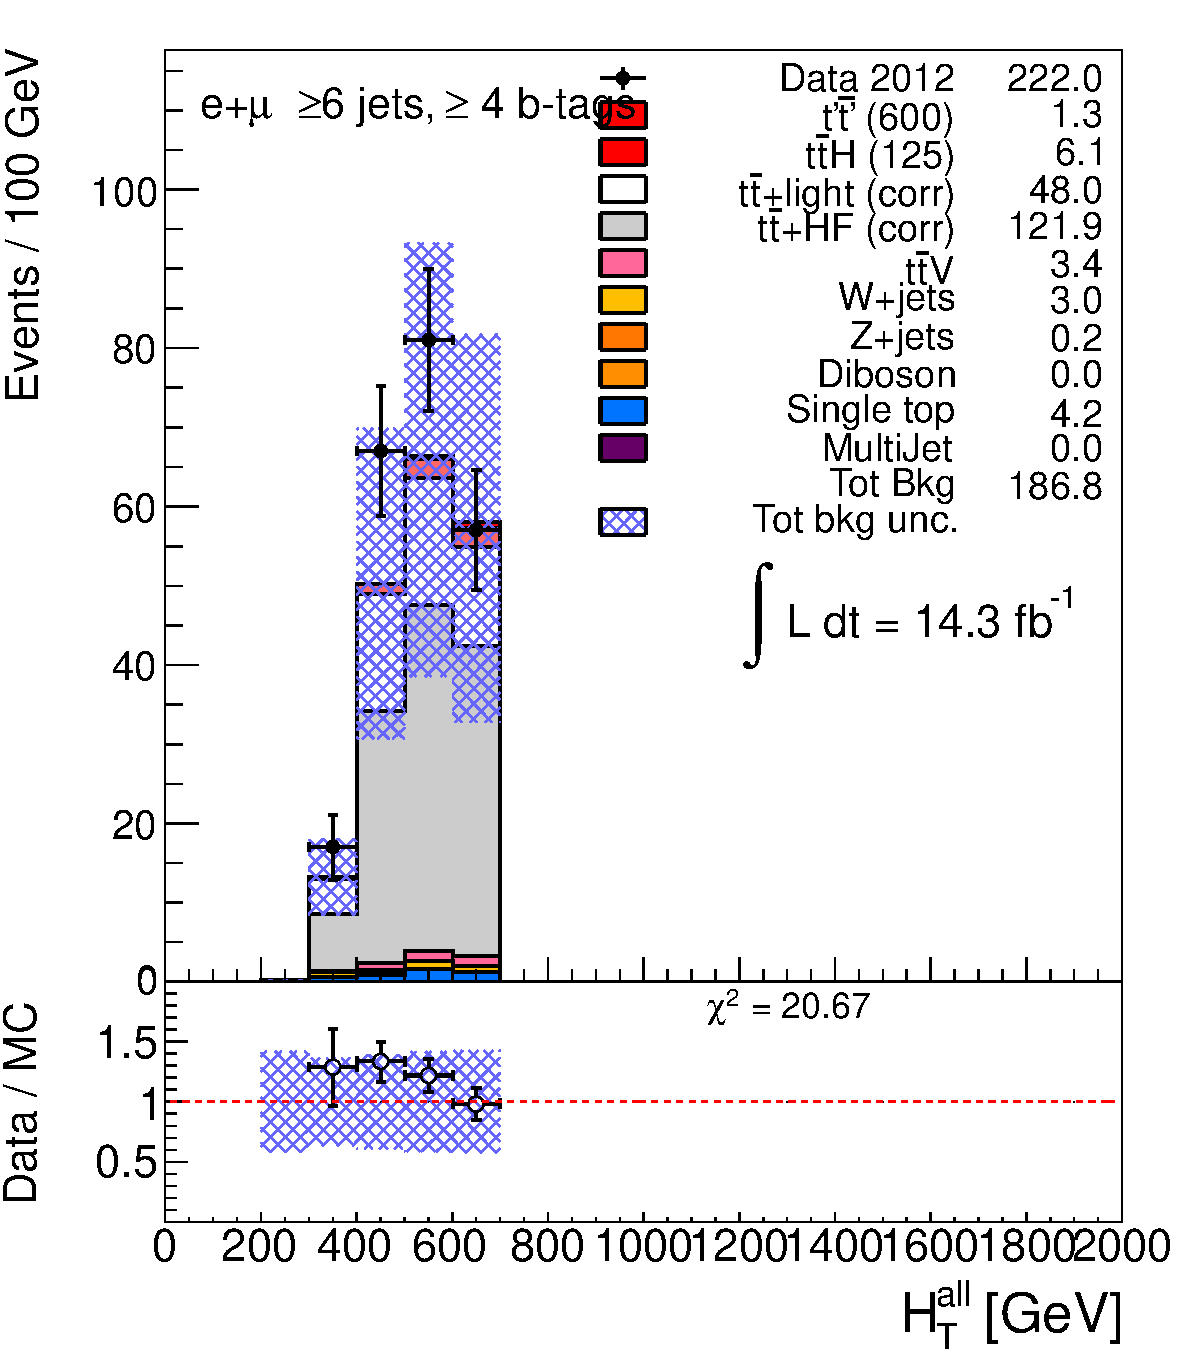
\includegraphics[width=.3\textwidth]{pics/htx_scaled/HTAll_ELEMUON_6jetin4btagin_NOMINAL.pdf}
%}\only<3>{
%final\\
%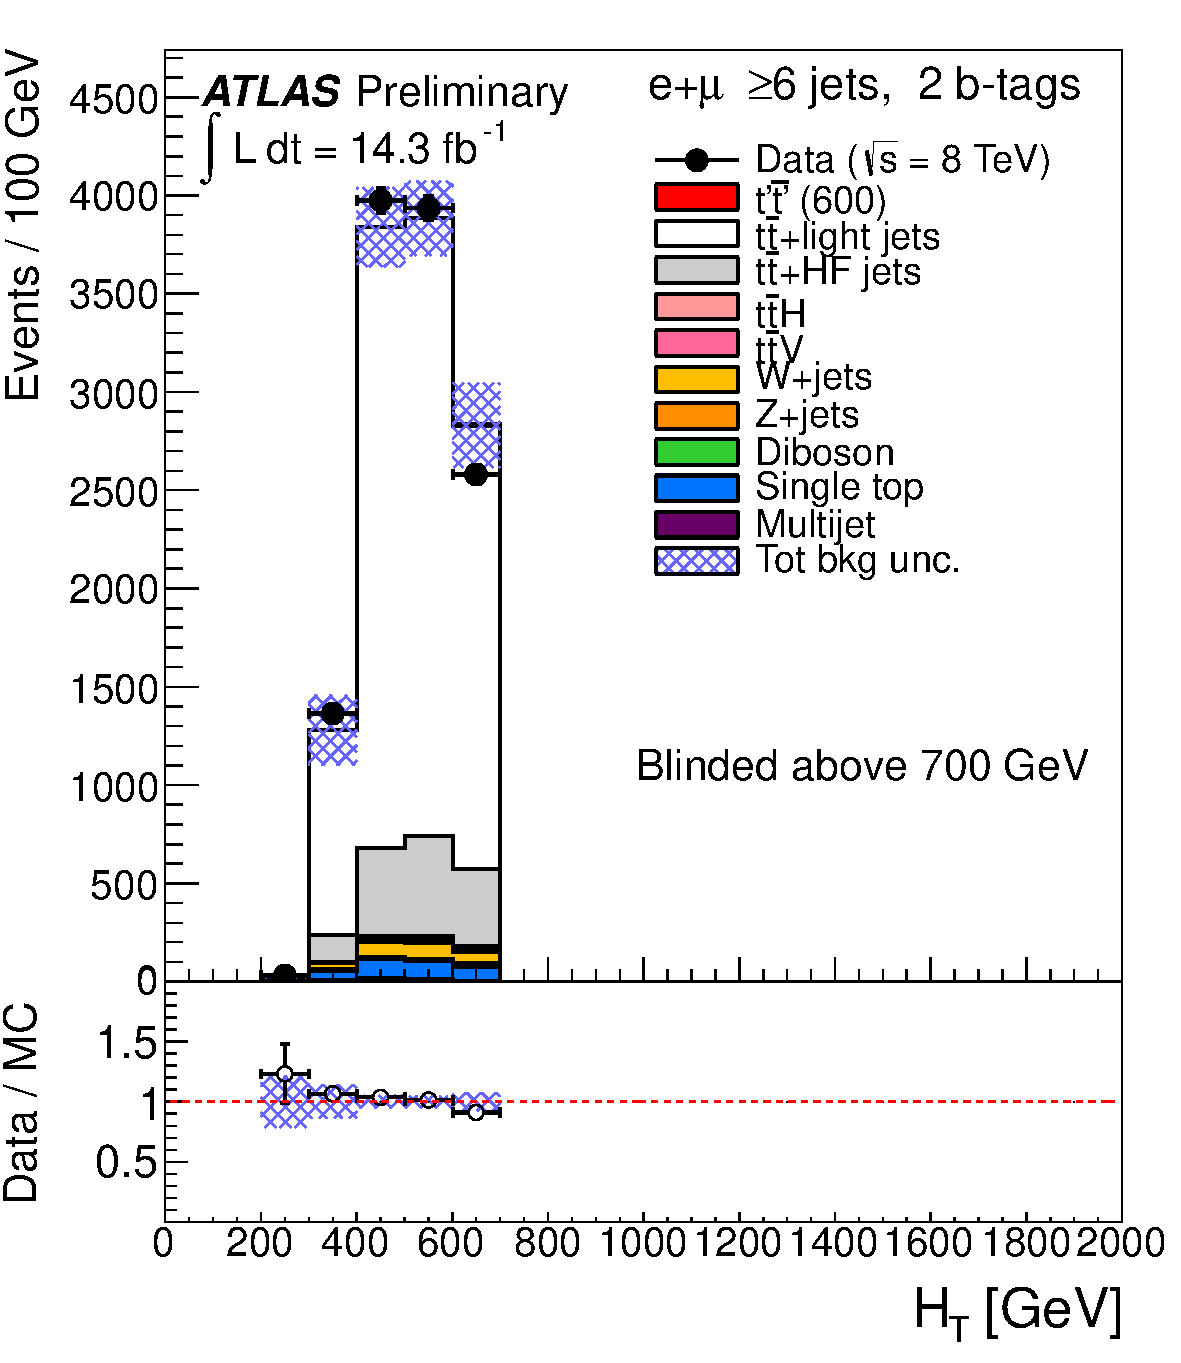
\includegraphics[width=.3\textwidth]{pics/htx_final/HTAll_6jetin2btagex_ELEMUON.pdf}
%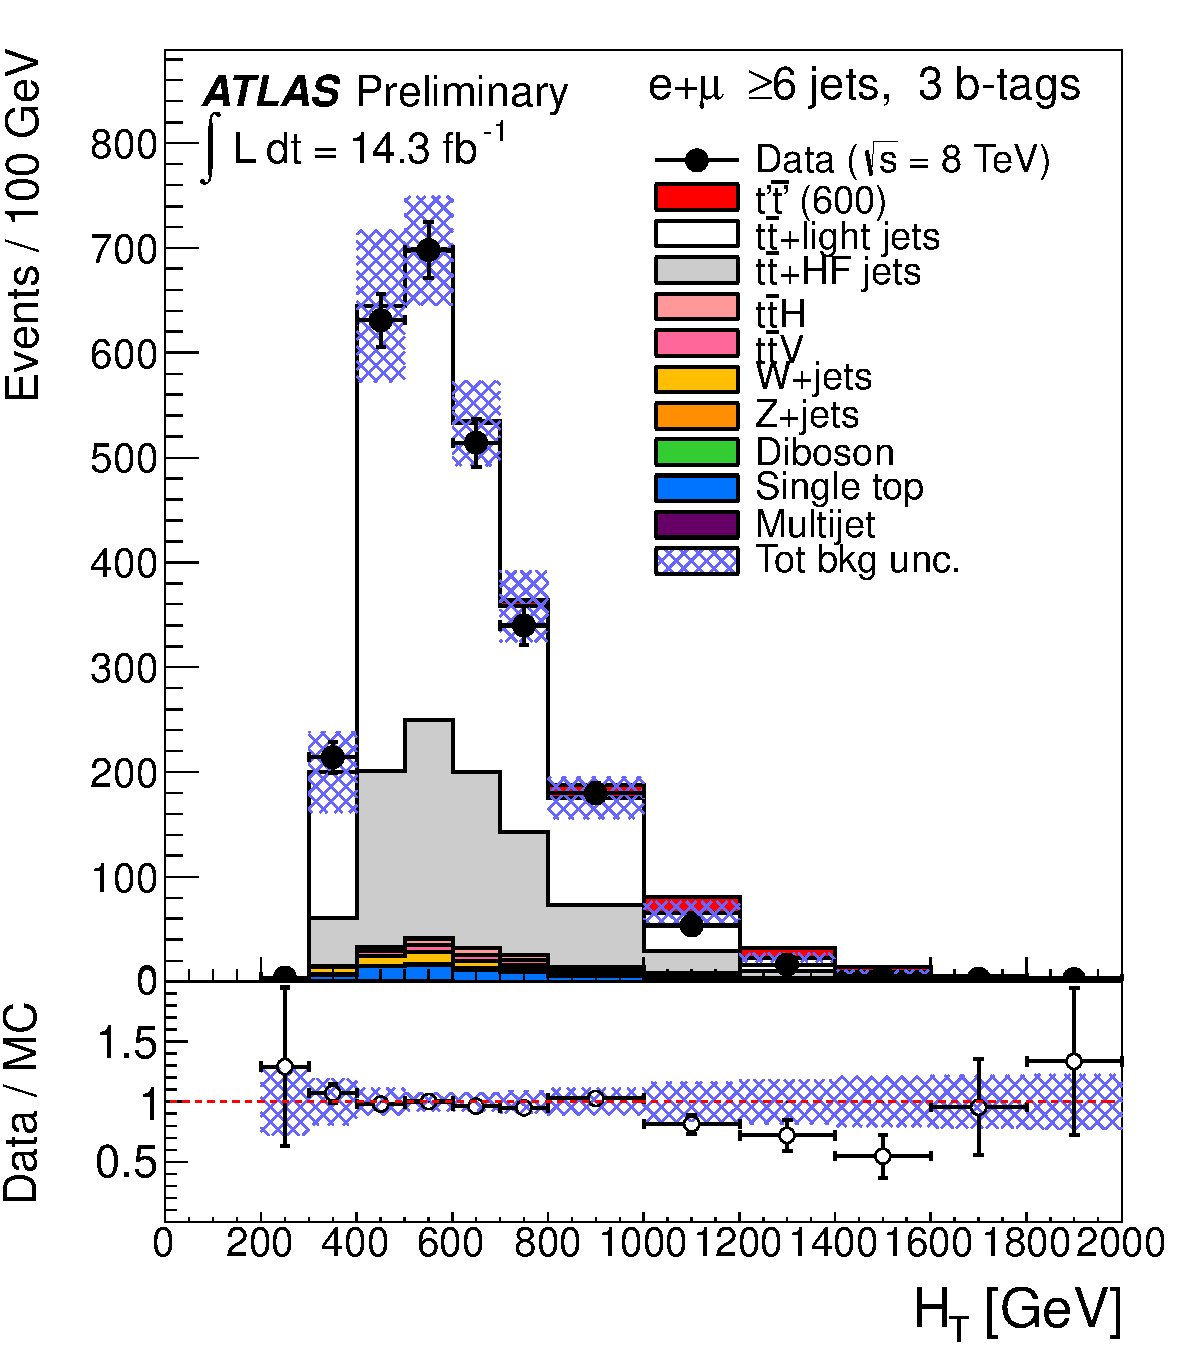
\includegraphics[width=.3\textwidth]{pics/htx_final/HTAll_6jetin3btagex_ELEMUON.pdf}
%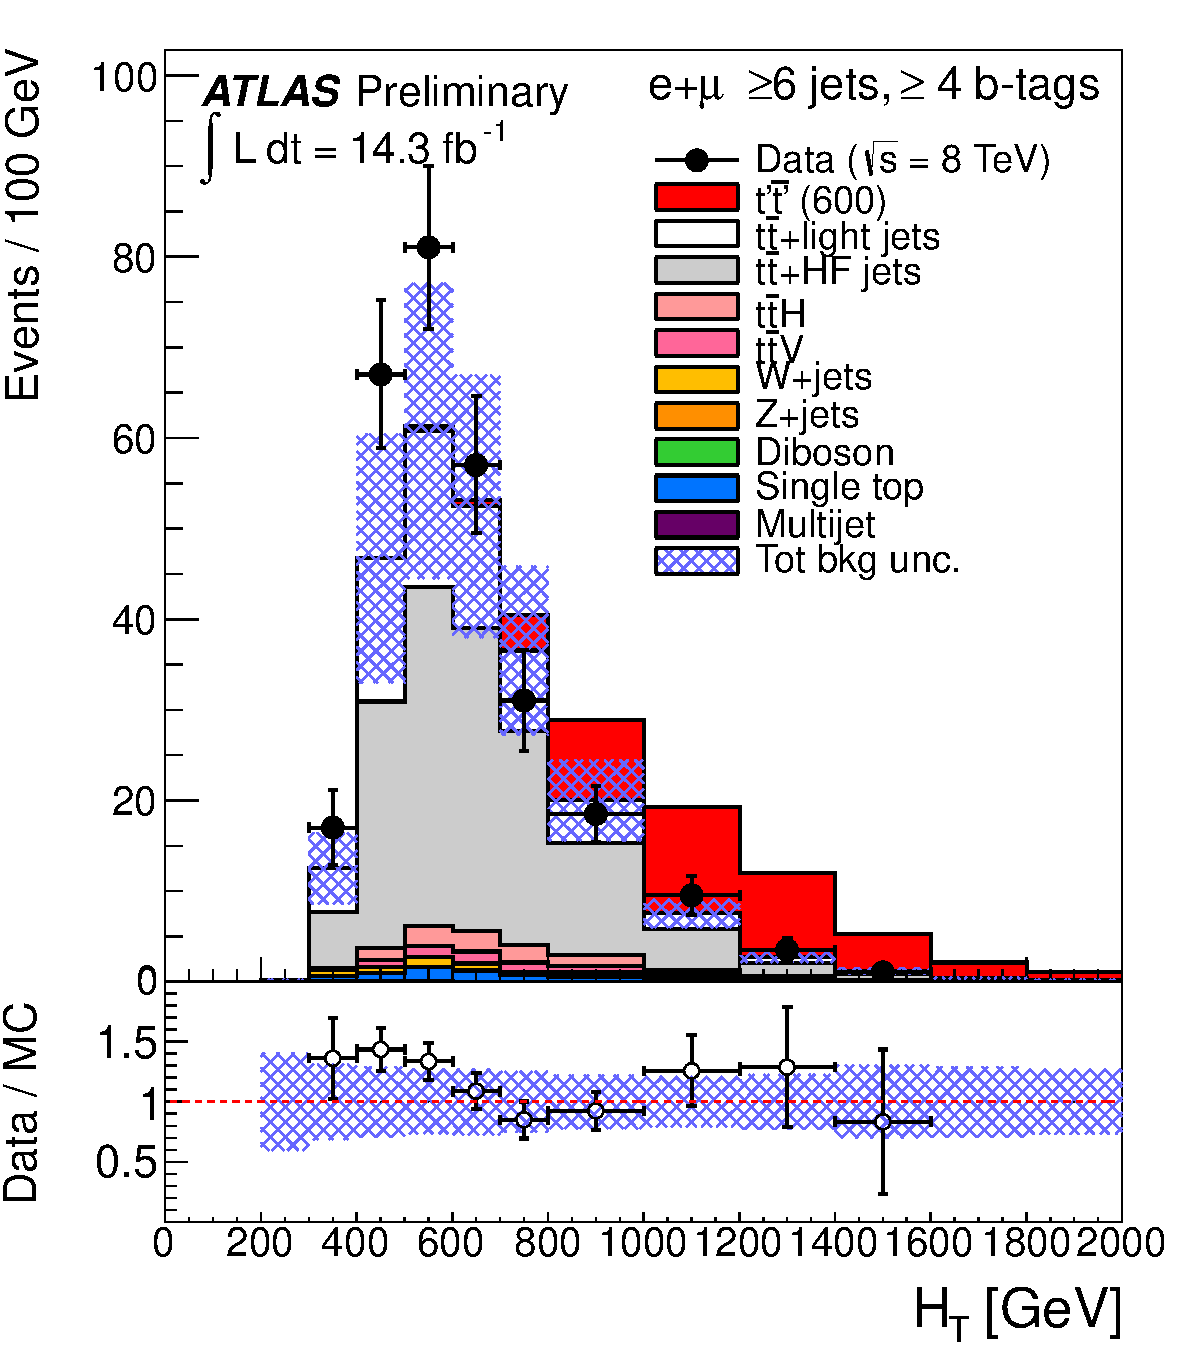
\includegraphics[width=.3\textwidth]{pics/htx_final/HTAll_6jetin4btagin_ELEMUON.pdf}
}

Maximum yields discrepancy below 5\%

\end{frame}


%%%%%%%%%%%%%%%%%%%%%%%%%
%%%
%%%%%%%%%%%%%%%%%%%%%%%%%
\begin{frame}\frametitle{Comparison data vs prediction}
\centering\footnotesize

Blinding cut: $\HT<700\gev$

{\Large$\Downarrow$}

Define special blinded regions to check \HT\ modeling:

\myskip

at most two jets with $\pt>60\gev$, $\HT<1.2\tev$

\begin{minipage}{.45\textwidth}\centering
 2 \btag ged jets\\
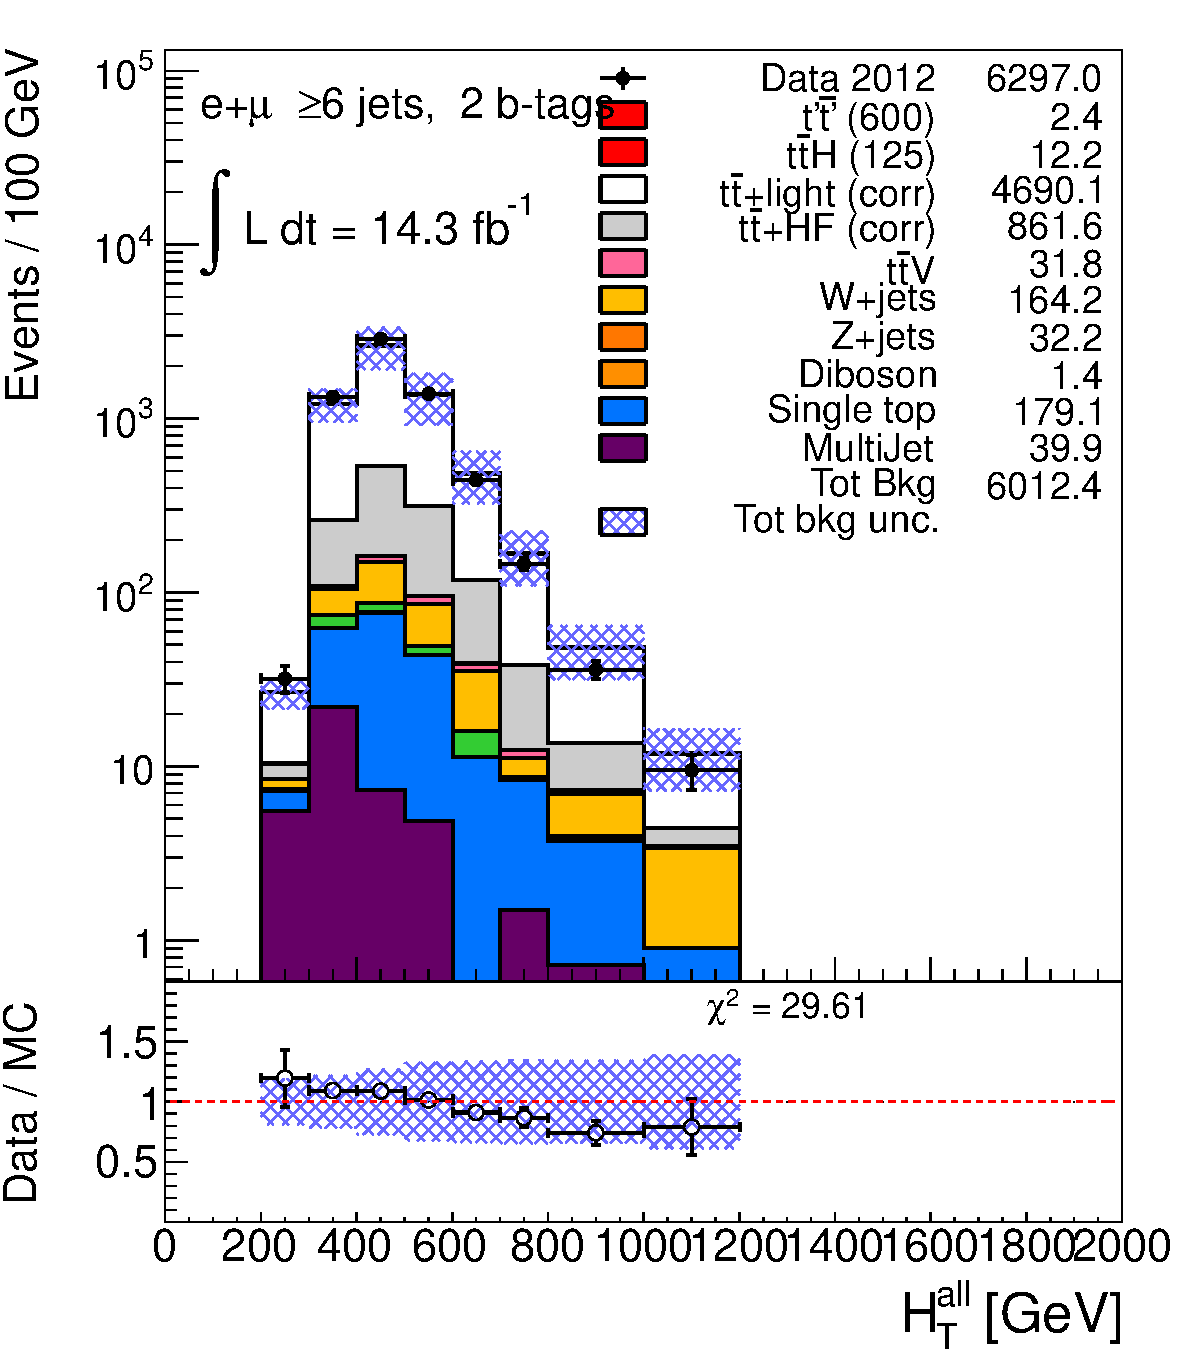
\includegraphics[width=.8\textwidth]{pics/htx_httails/HTAll_ELEMUON_6jetin2btagex_NOMINAL_logscale}

\end{minipage}\begin{minipage}{.45\textwidth}\centering

 3 \btag ged jets\\
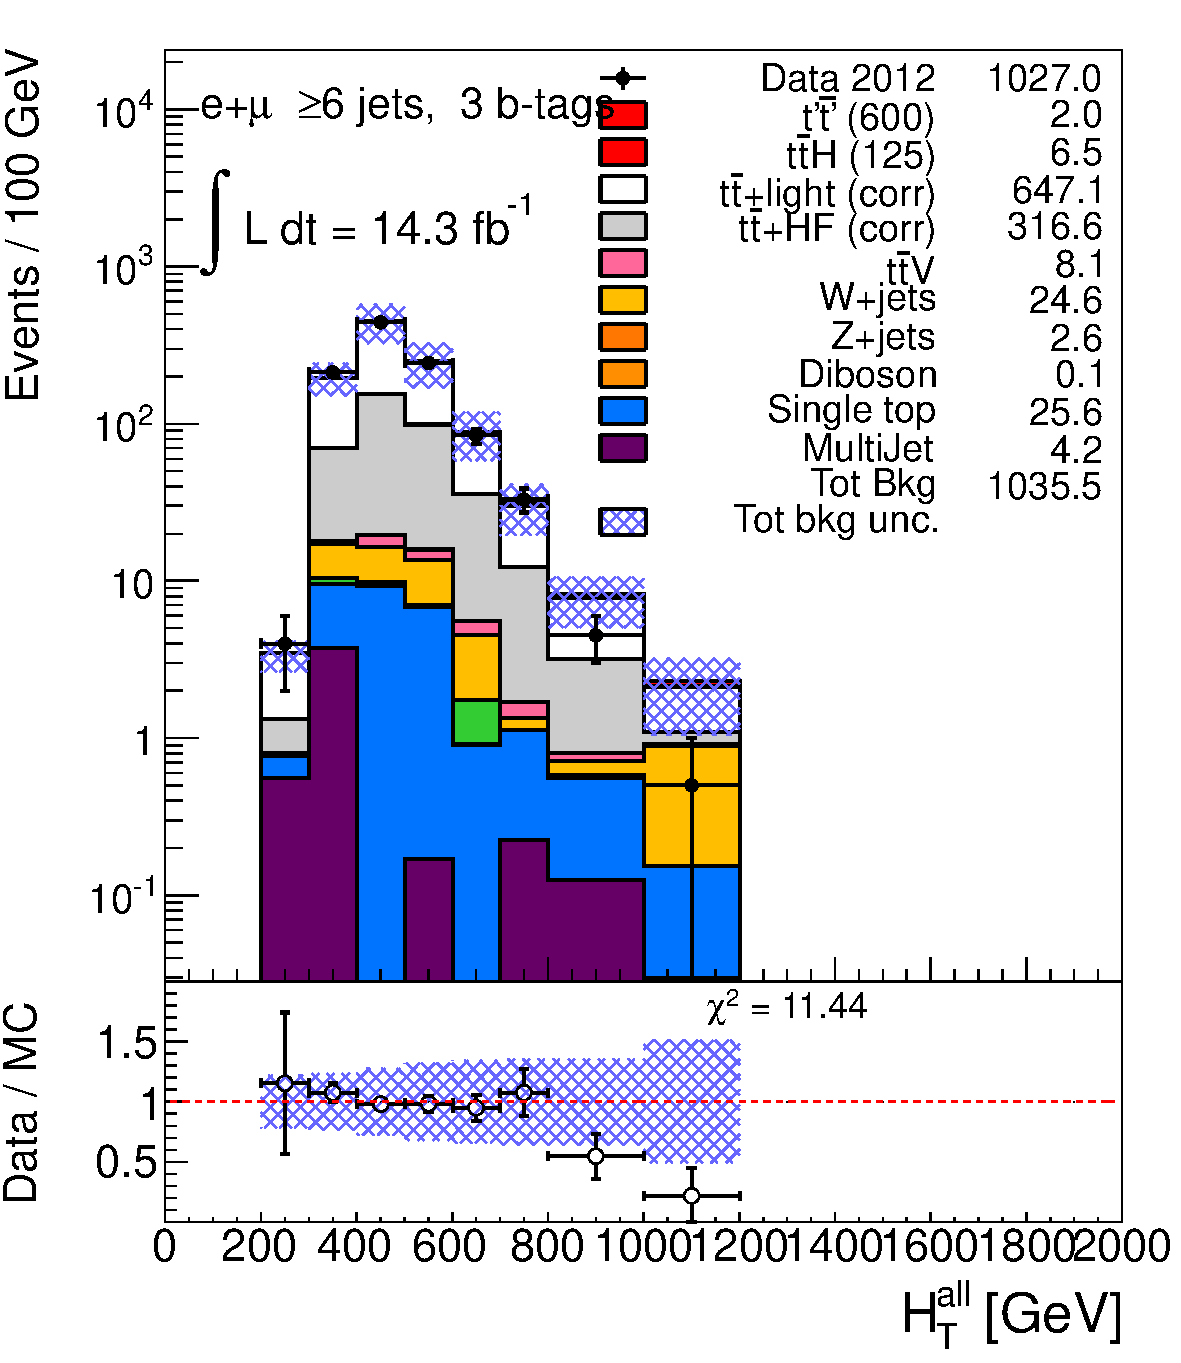
\includegraphics[width=.8\textwidth]{pics/htx_httails/HTAll_ELEMUON_6jetin3btagex_NOMINAL_logscale}

\end{minipage}

\end{frame}



%%%%%%%%%%%%%%%%%%%%%%%%%
%%%
%%%%%%%%%%%%%%%%%%%%%%%%%
\begin{frame}\frametitle{Most relevant systematic uncertainties}
\centering\footnotesize

\ttbar\ modeling systematics:
\begin{itemize}
\item Vary the original and the dynamic factorization scales (``qfac'' and ``iqopt2'')
\item Vary the renormalization scale (``ktfac'')
\end{itemize}

\myskip

{
\scriptsize
\begin{tabular}{l*{4}{c}}\toprule
 & \TTbar & $t\bar{t}$-HF & $t\bar{t}$-Light \\
\midrule
Total [\%]& +21.9/-24.0 & +57.3/-58.4 & +42.0/-44.1 \\
\midrule
\multicolumn{4}{c}{Main contributions [\%]}\\
BTAGBREAK8 & +20.4/-22.7 & +15.8/-17.8 & +12.2/-13.1 \\
JES ``baseline'' & +3.1/-3.1 & +10.5/-10.5 & +13.7/-13.7 \\
ttbar iqopt2 & -- & +6.9/-6.9 & +20.1/-20.1 \\
ttbar ktfac & -- & +7.5/-9.2 & +13.8/-17.0 \\
ttbar qfac & -- & +0.7/-0.7 & +1.6/-1.6 \\
ttbarHF & -- &+50.0/-50.0 & +13.0/-13.0 \\
\bottomrule
\end{tabular}
}

\myskip

Introduce the scaling factors as {\cccolor nuisance parameters}\\
{\Large $\Downarrow$}\\
total uncertainty on \tthf\ reduced by $\sim 20$\% 
%{\cccolor \dots before fitting the nuisance parameters}

\end{frame}


%%%%%%%%%%%%%%%%%%%%%%%%%
%%%
%%%%%%%%%%%%%%%%%%%%%%%%%
\begin{frame}\frametitle{Yields in signal regions}
\centering\scriptsize

\myskip
\begin{minipage}{.5\textwidth}\centering

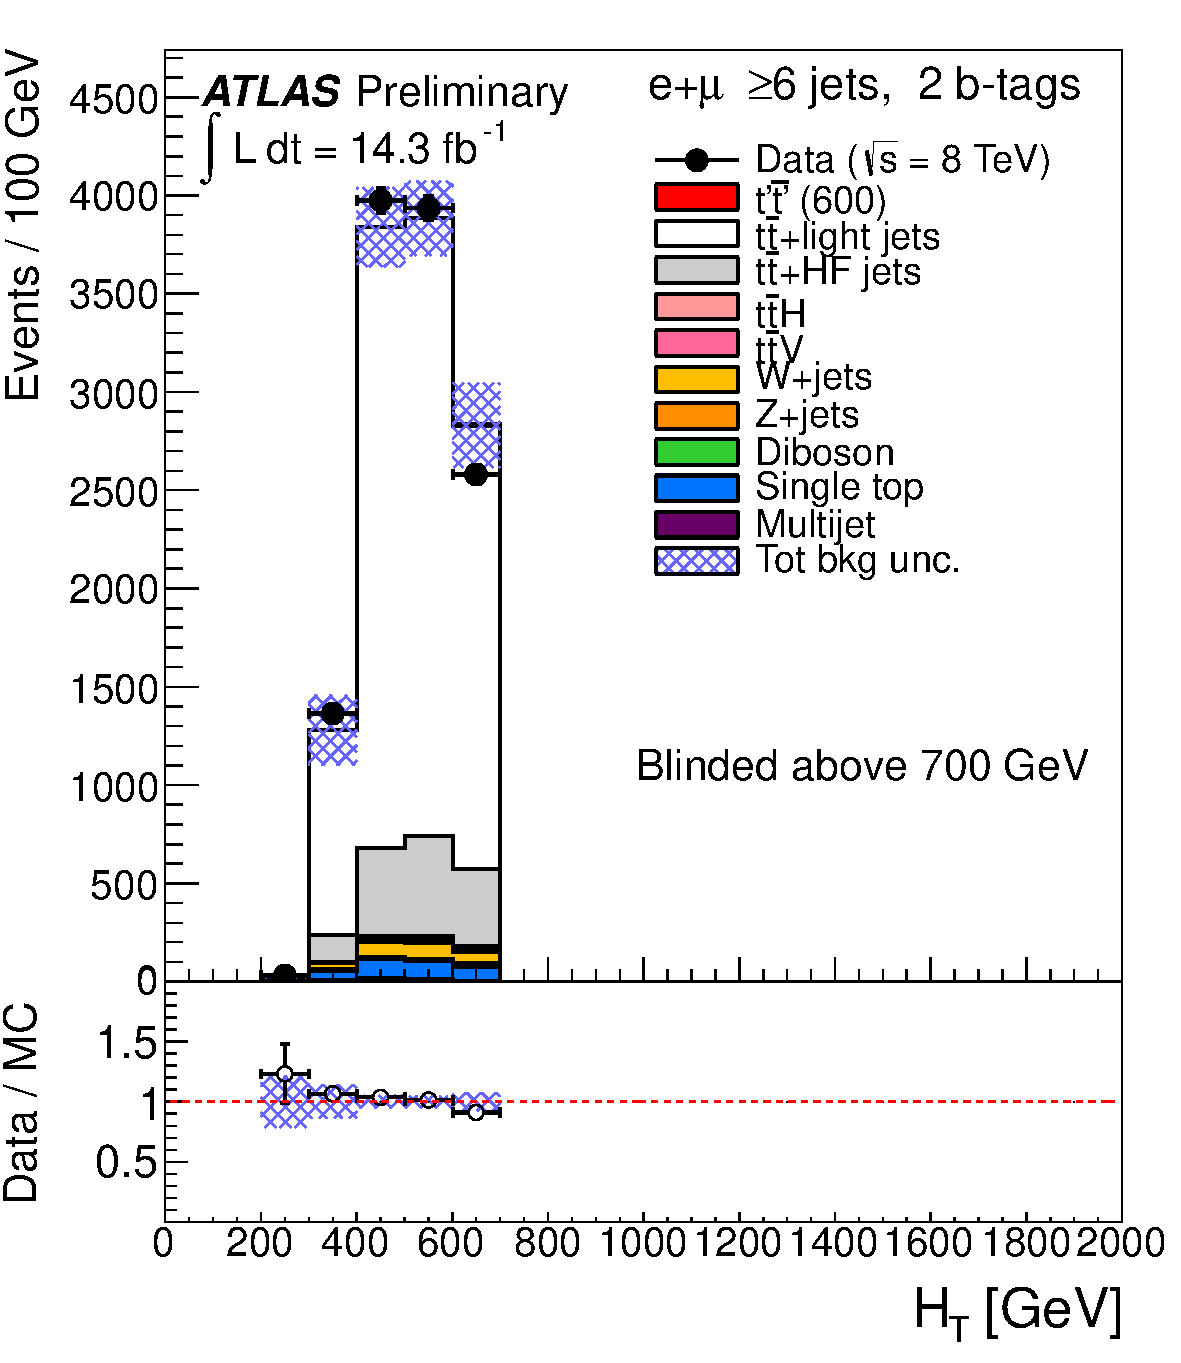
\includegraphics[width=.5\textwidth]{pics/htx_final/HTAll_6jetin2btagex_ELEMUON.pdf}
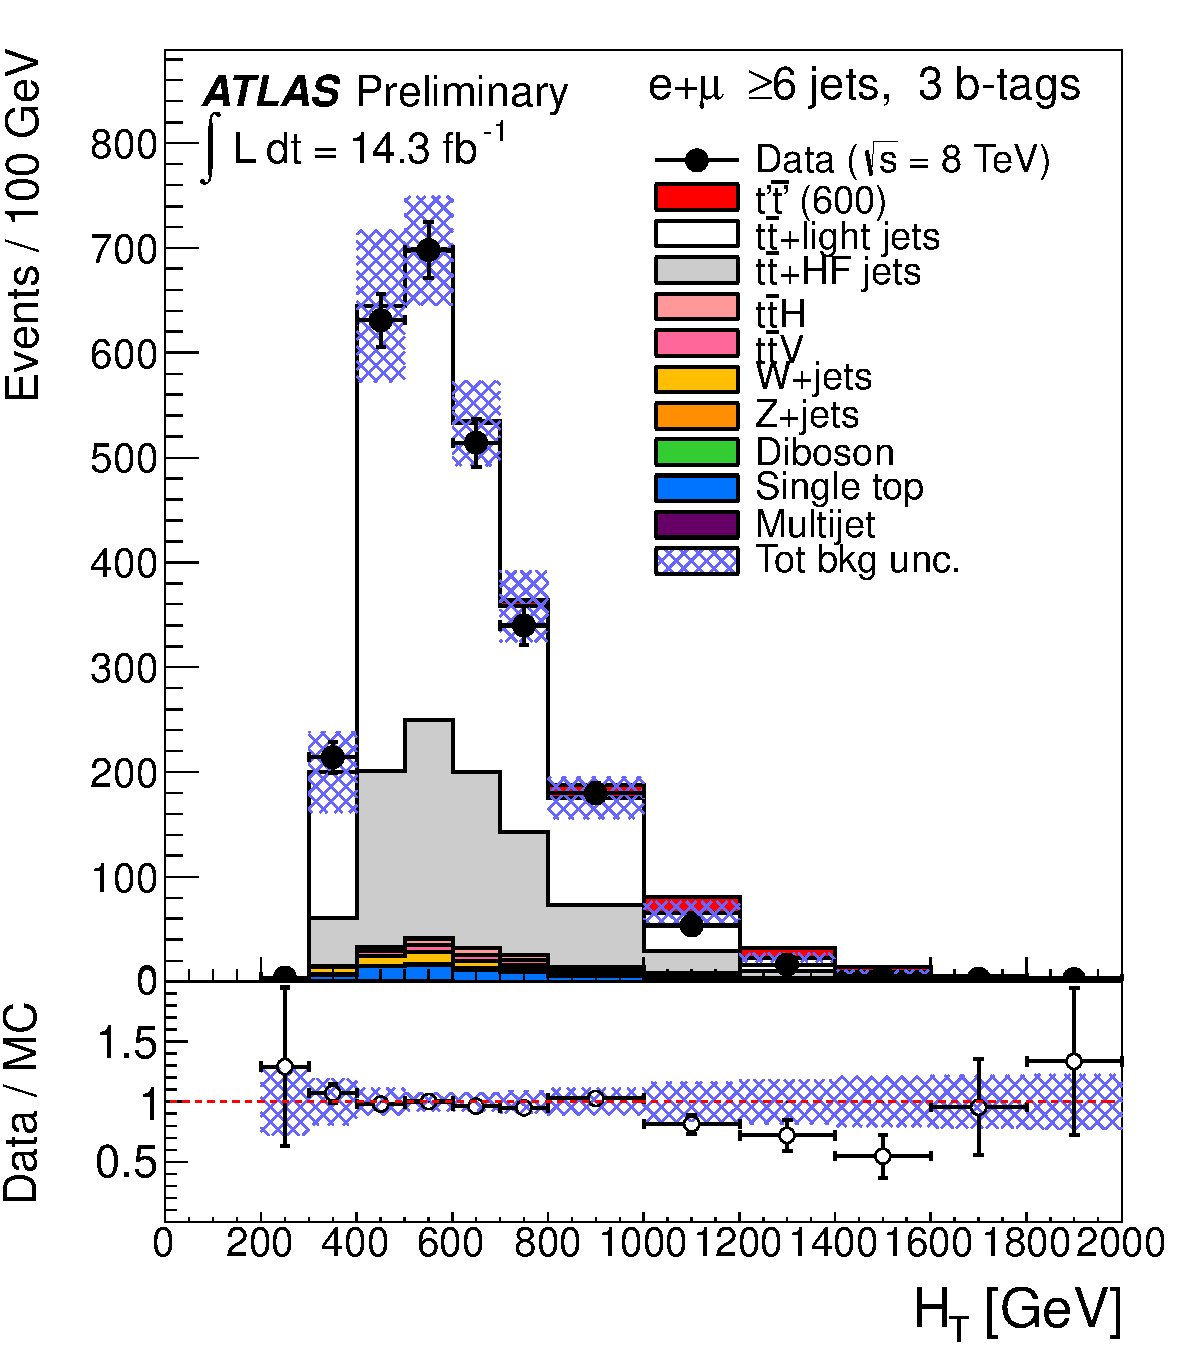
\includegraphics[width=.5\textwidth]{pics/htx_final/HTAll_6jetin3btagex_ELEMUON.pdf}

%\resizebox{.9\textwidth}{.25\textwidth}{
\resizebox{.9\textwidth}{!}{
\begin{tabular}{l D{;}{\,\pm\,}{-1} D{;}{\,\pm\,}{-1} D{;}{\,\pm\,}{-1}} \toprule
 & \multicolumn{1}{c}{ 2 $b$-tags} & \multicolumn{1}{c}{ 3 $b$-tags} & \multicolumn{1}{c}{ $\geq$ 4 $b$-tags}\\
\midrule
$t\bar{t}$+HF  &  1500;900 &  900;400 &  170;70\\
$t\bar{t}$+LF  &  9600;1000 &  1900;350 &  75;22\\
$W$+jets  &  250;130 &  50;30 &  5;3\\
$Z$+jets  &  50;40 &  9;6 &  0.5;0.9\\
Single top  &  300;70 &  75;18 &  7;3\\
Diboson  &  1.7;0.6 &  0.3;0.1 &  0.03;0.03\\
$t\bar{t}V$ & 70;20 &  36;12 &  7;3\\
$t\bar{t}H$ & 28;4 &  31;6 &  12;3\\
Multijet  &  49;23 &  1.7;0.8 &  0.15;0.06\\
\midrule
Tot.Bkg.  &  11860 ;260 &  2990;210 &  270;60\\
Data & \multicolumn{1}{c}{11885} & \multicolumn{1}{c}{2922} & \multicolumn{1}{c}{318}\\
\midrule
%\multicolumn{7}{l}{Doublet}\\
%\midrule
$T\bar{T}$ (600) & & & \\
doublet &  4.3;1.2 &  94;7 &  79;18\\
singlet  &  2.3;0.4 &  61;7 &  36;9\\
%T\bar{T} (400);550;70 &  1100;100 &  790;160\\
%T\bar{T} (600);4.3;1.2 &  94;7 &  79;18\\
%T\bar{T} (800);0.12;0.05 &  10.7  & 0.8 &  9.1;2.1\\
%\midrule
%\multicolumn{7}{l}{Singlet}\\
%\midrule
%T\bar{T} (400);290;30 &  650;80 &  330;70\\
%T\bar{T} (600);2.3;0.4 &  61;7 &  36;9\\
%T\bar{T} (800);0.06;0.01 &  6.9;0.7 &  4.2;1.1\\
\bottomrule
\end{tabular}
}

\myskip

\footnotesize

\end{minipage}\begin{minipage}{.5\textwidth}\centering

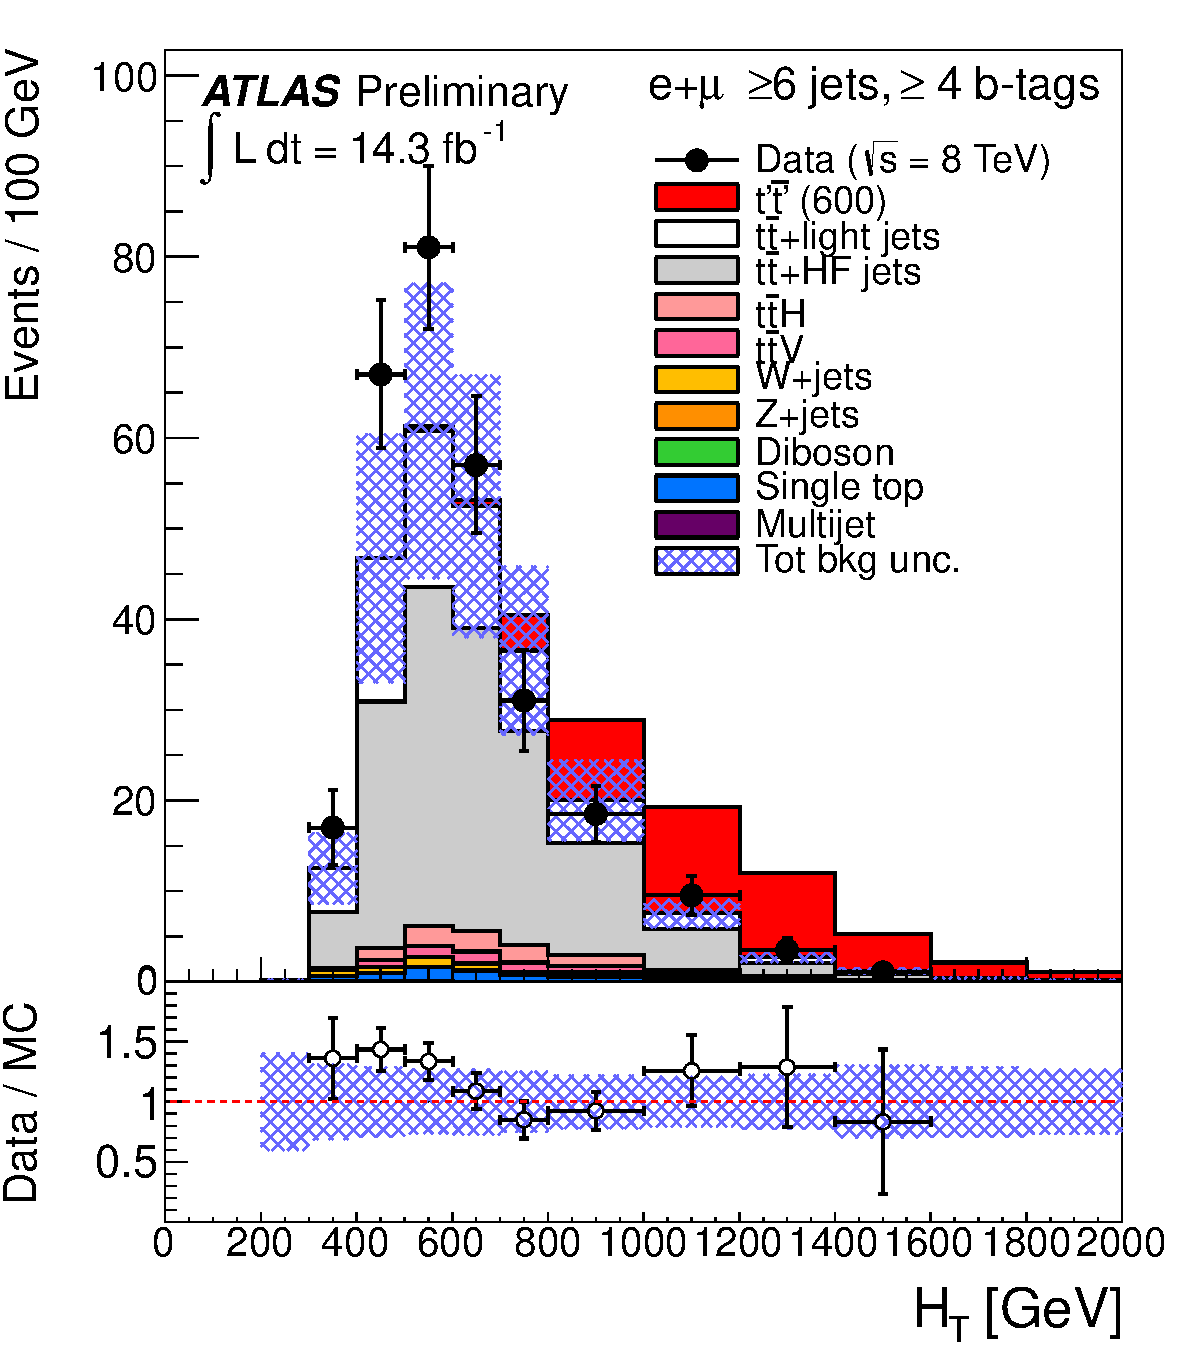
\includegraphics[width=.9\textwidth]{pics/htx_final/HTAll_6jetin4btagin_ELEMUON}

\end{minipage}

\end{frame}


%%%%%%%%%%%%%%%%%%%%%%%%%
%%%
%%%%%%%%%%%%%%%%%%%%%%%%%
\begin{frame}\frametitle{Benchmark results}
\centering\footnotesize

\begin{minipage}{.5\textwidth}\centering

Doublet\\

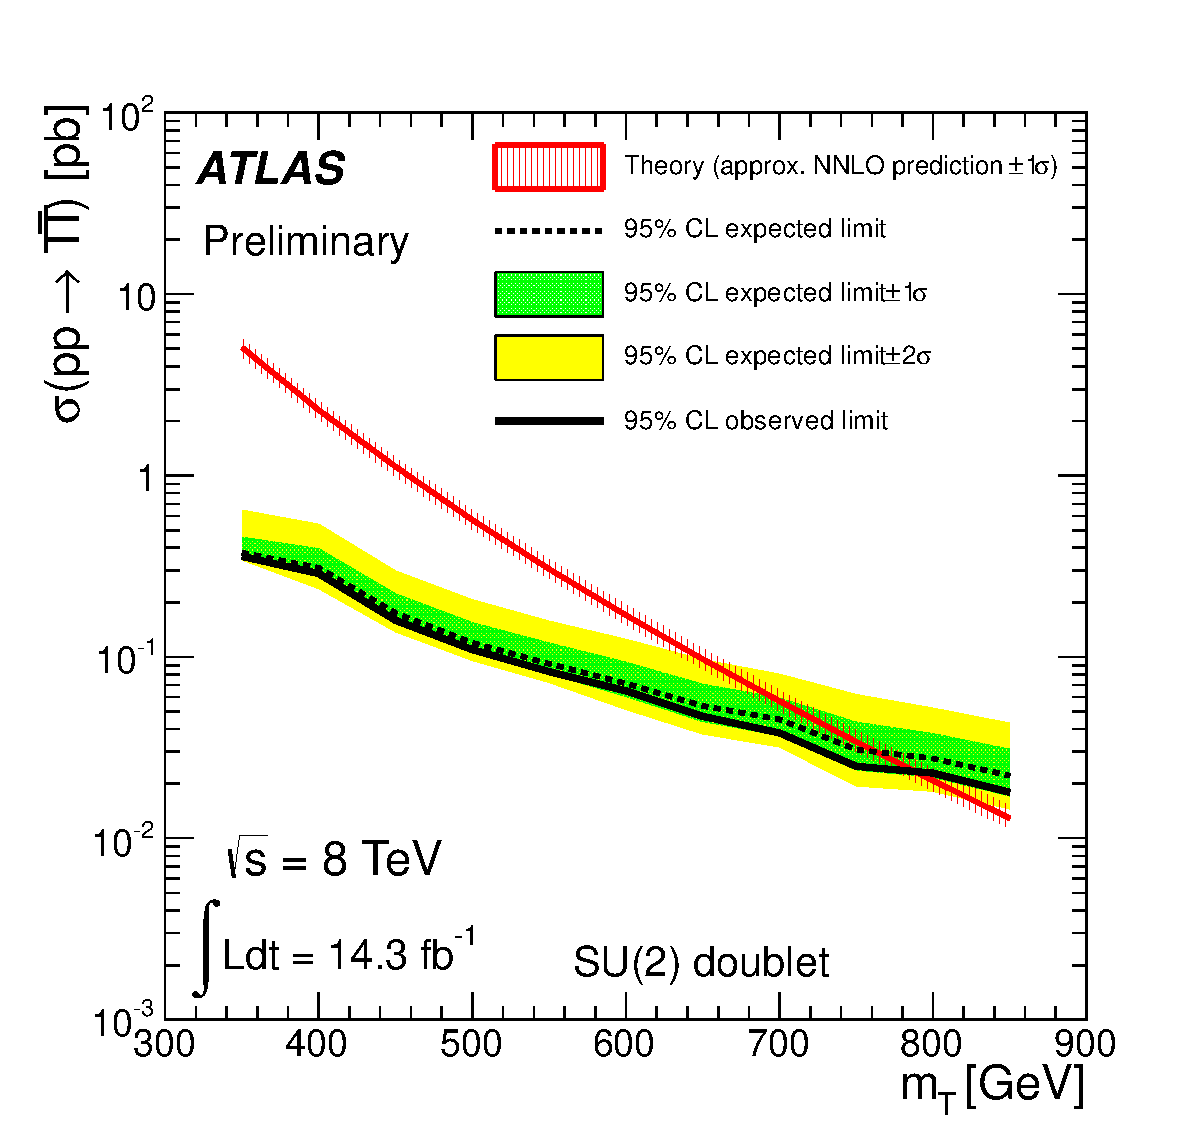
\includegraphics[width=0.9\textwidth]{pics/lim_doublet}\\

observed (expected) 95\%  CL limit $m_{T}>790\,(745)\gev$

\end{minipage}\begin{minipage}{.5\textwidth}\centering

Singlet\\

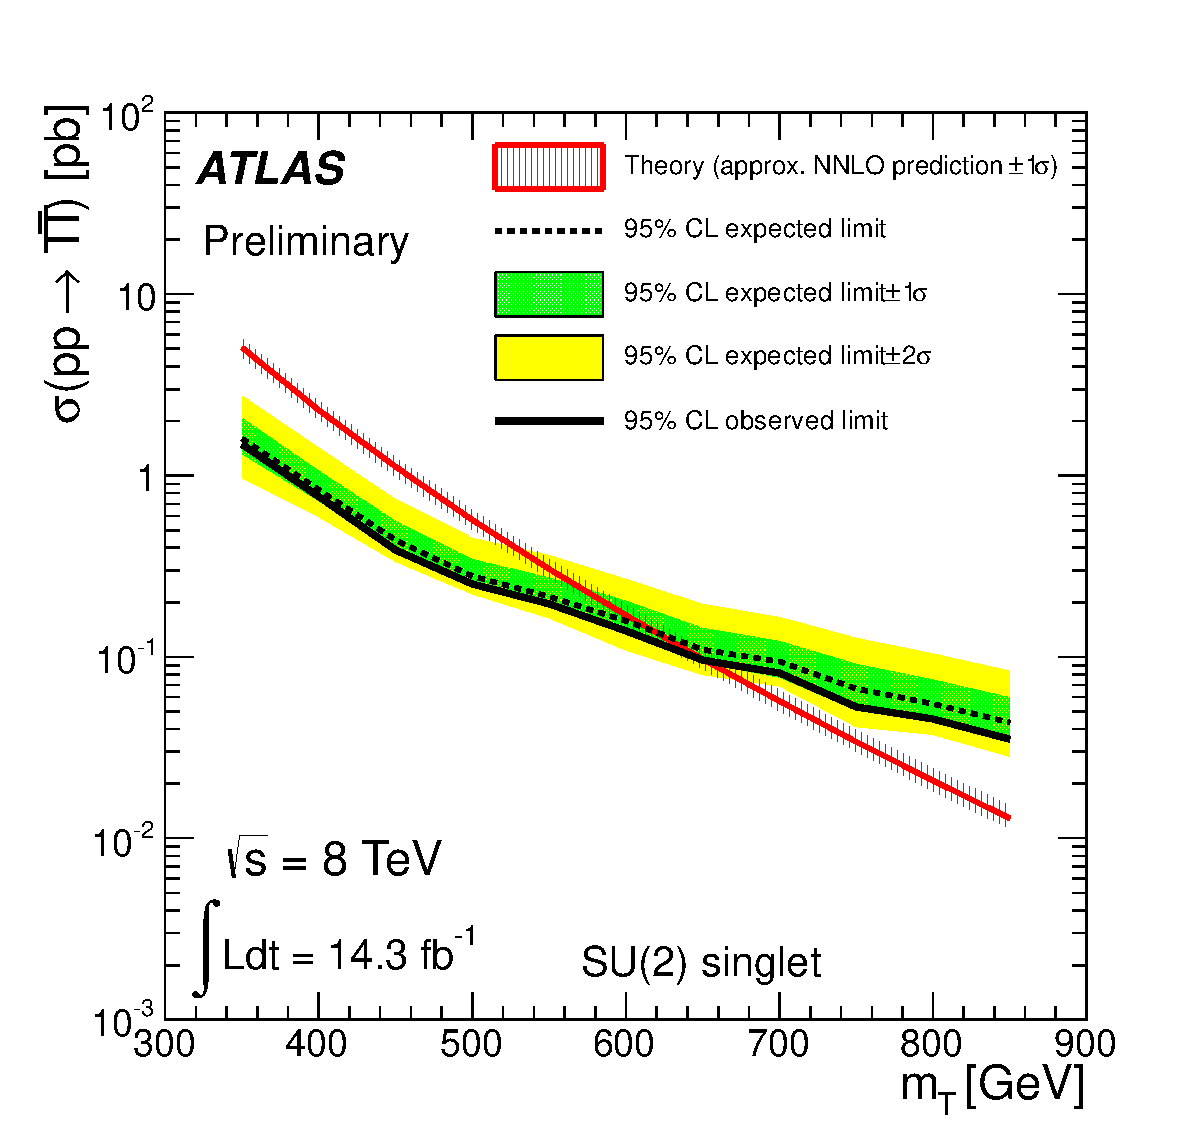
\includegraphics[width=0.9\textwidth]{pics/lim_singlet}\\

observed (expected) 95\%  CL  limit  $m_{\T}>640\,(615)\gev$

\end{minipage}

\end{frame}

%%%%%%%%%%%%%%%%%%%%%%%%%
%%%
%%%%%%%%%%%%%%%%%%%%%%%%%
\begin{frame}\frametitle{Model independent results}
\centering\footnotesize

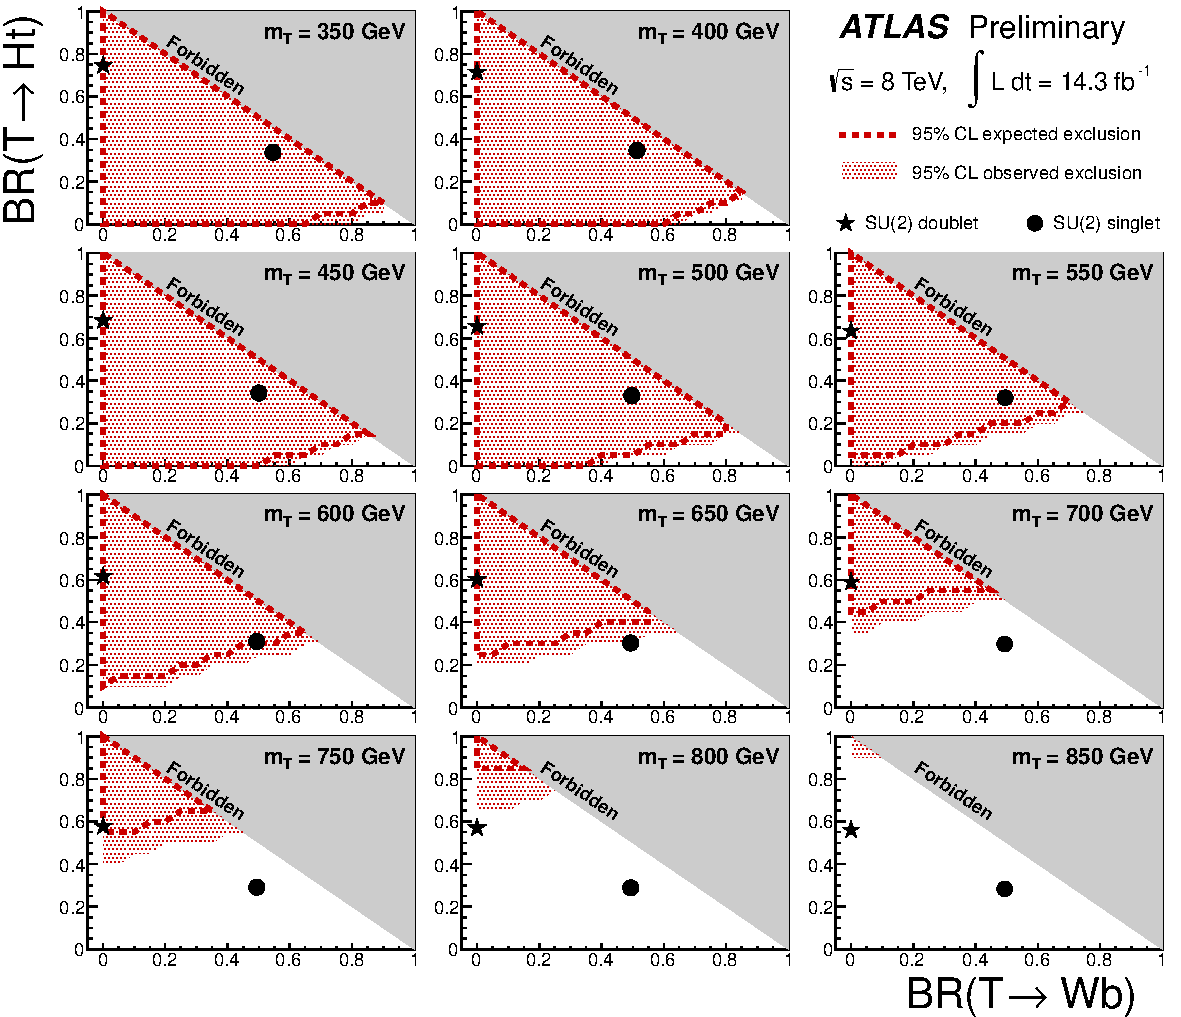
\includegraphics[width=0.7\textwidth]{pics/lim_2D}

\end{frame}



